%%%%%%%%%%%%%%%%%%%%%%%%%%%%%%%%%%%%%%%%%
% SC Information Paper 5 
% SHARK INDICATORS IN THE WESTERN CENTRAL PACIFIC
% June 2015
%
% Author: Joel Rice (joelrice@uw.edu )
%
%
%%%%%%%%%%%%%%%%%%%%%%%%%%%%%%%%%%%%%%%%%

%----------------------------------------------------------------------------------------
%  PACKAGES AND OTHER DOCUMENT CONFIGURATIONS
%----------------------------------------------------------------------------------------
\documentclass[12pt]{SCreport}

\graphicspath{ {C:/Projects/SHK-indicators-2015/GRAPHICS/} {C:/Projects/SHK-indicators-2015/GRAPHICS/Defined/} {C:/Projects/SHK-indicators-2015/GRAPHICS/CPUE_std/} }

\usepackage[english]{babel}


%\documentclass[12pt]{SCreport}
\newtoggle{includefigs}
%\togglefalse{includefigs} % to include figures, uncomment \toggletrue{includefigs} 
%\usepackage{graphicx} 
\usepackage{multirow} 
\usepackage{array} 
%\usepackage{lscape} 
%\usepackage{caption} 
\usepackage{subcaption}

\toggletrue{includefigs}


  \reportauthor{Joel Rice\footnote{Joel Rice Consulting Ltd.}, Laura Tremblay-Boyer, Shelton Harley, Robert Scott, Steven Hare and Alex Tidd}
  \reporttitle{Analysis of stock status and related indicators for key shark species of the Western Central Pacific Fisheries Commission}
  \reportnumber{EB-WP-04}

\usepackage{grffile}

%----------------------------------------------------------------------------------------
%  Document content
%----------------------------------------------------------------------------------------

\begin{document}

\wcpfctitlepage

\tableofcontents

\newpage
\section*{Executive Summary}
In this report we present, for seven of the fourteen key shark species, information on the geographic range of catches; temporal trends in catch composition and catch rates; and key biological indicators of fishing pressure such as mean size and sex ratio. Whale sharks are assessed separately due to the unique nature of their interactions with WCPO fisheries. The analysis generally follows the framework first developed and described in the Shark Research Plan (SC6; Clarke and Harley 2010). 

This analysis provides indicative trends for silky shark, oceanic whitetip, mako shark, blue shark, whale sharks and porbeagle sharks, but more limited inferences are  possible for hammerhead and thresher sharks, largely due to lack of data. These species are not commonly caught in the primary fisheries in the WCPO, and are historically not well reported. 

\textbf{Species occurrence indicators} show that five of the seven species are encountered across the breadth of the WCPFC region. The exceptions are hammerheads, which are distributed more patchily, and porbeagle which are restricted to the region south of 20\degree{}S. The proportion-presence and High-CPUE indicators showed relatively steady trends for most species in all regions. However, for blue shark and oceanic whitetip sharks both indicators show declines as great as 80\% in Regions 3 through 6.

\textbf{Species Composition indicators} reveal that shark bycatch differs substantially between longline and purse seine fishing in the WCPO. Blue sharks are the most prevalent longline caught shark, and silky shark are the second most common. There are substantial regional and depth variations.  Several species are caught more frequently in deeper sets, while porbeagle form a sizeable component of the shallow sets in the regions where they occur (i.e., Regions 5 and 6). Purse seine shark bycatch has much lower species diversity and is dominated by silky sharks, which generally comprise more than 95\% of the shark bycatch. Minor numbers of hammerhead and oceanic whitetip sharks also occur.  

\textbf{CPUE indicators} indicate that blue shark CPUE is declining in both the north and south Pacific. Oceanic white tip continue to decline throughout the tropical waters of the WCPO. Silky shark CPUE exhibits high fluctuations throughout the study period.  
CPUE for the thresher shark complex, and Mako sharks in the south Pacific, appear to be in decline, though the last years' data points are based on relatively few data.  
Mako in the north Pacific is subject to missing data for some years; trends in CPUE appeared relatively stable between 2000 and 2010, but no inference is possible for the last 4 years. Porbeagle shark CPUE experienced a large decrease early on in the study period followed by a fluctuating but increasing CPUE trend.


\textbf{Biological Indicators} show that the sex ratio of sharks in longline catch is approximately equal for all species and regions, with the exception of blue shark in Region 5, which are predominantly female.
 The majority of the observed hammerhead, silky, thresher, oceanic whitetip and porbeagle sharks were immature. Observed blue shark were mainly immature in Regions 5 and 6, and mature in Region 2. Declines in standardised annual lengths are apparent in most regions for most species, with annual declines of 0.2-0.4 cm/yr.
The largest decline was seen for the southern stock of male mako sharks, which have declined by 0.6 cm/yr. By contrast slight increases in annual standardised length were seen for northern mako sharks (both sexes).


\subsection*{Recommendations to the Scientific Committee}
Based on the indicators examined in this analysis, we invite the SC to consider the following recommendations when considering future research priorities: 
 
 \begin{itemize}
\item Increased observer monitoring is vital to provide improved information for all shark species to support development of stock assessments as well as gather fishery information necessary to monitor the impact of CMMs.   
 
\item Research to assess the discrepancy between shark reporting in logbooks and observer data.  

\item Silky shark and oceanic whitetip sharks have been declining under recent fishing pressure, and likely maintain their overfished status. While updated assessments may be warranted for both stocks, this would appear most useful for silky shark to understand how its stock status has changed in recent years in conjunction with the new CMMs. 

\item Stock assessments for blue sharks in the south Pacific, mako sharks, oceanic whitetip sharks (in the WCPO and Pacific wide) and silky sharks should be scheduled within the next five years.   

\item An investigation of the initial depletion levels for assessed shark stocks should be undertaken, including the development of catch histories. 

\item For currently unassessed stocks, the development of catch histories would enable more informative analyses in future. For hammerhead and thresher sharks the analysis of catch species composition would be similarly useful.

\item  For silky, oceanic whitetip and whale sharks, information on post release mortality rates is needed to monitor the effectiveness of existing non-retention management measures. This work requires an update to the information collected by observers with respect to shark releases; to this end an update to observer forms and data collection procedures will be required. 

\item A similar indicator analysis be undertaken for relevant key shark species again in 2-3 years with a stock assessment for blue shark in the south Pacific, and another silky shark assessment conducted in the interim. 

\end{itemize}



%\end{itemize}






\newpage
\section{Introduction} % ltb rev 90% done


Sharks are typically caught as bycatch in the Pacific tuna fisheries, though some directed and/or mixed species fisheries also exist. The Western and Central Pacific Fisheries Commission (WCPFC) has 14 designated key shark species (Table 1). Initially the list included blue shark, oceanic whitetip shark, mako sharks and thresher sharks. Silky, porbeagle (south of 30\degree{}S), hammerhead sharks (winghead, scalloped, great, and smooth) and whale sharks were added later.  The status of the five of these species (blue, mako, thresher, silky, and oceanic whitetip sharks) in the Western and Central Pacific Ocean (WCPO) was reviewed in 2011 \citep{Clarke2011_a, Clarke2011_b}. That review presented a number of indicators to inform on the status of the stock of these shark species and their response to fishing pressure. Given the paucity of data availability for sharks compared to target species, the indicators developed were based on data from logsheets and observer records from industrial purse-seine and longline vessels.

The current study updates key indicators and extends the analyses to include hammerhead, porbeagle and whale sharks. This study covers the time period 1995-2014. While some observer and logbook data exist for years prior to 1995, the majority of records either do not report shark catch or list it as a general category ‘shark’. At the time of analysis, sufficient data for 2014 were available both in logsheets and the observer data, however, the most recent observer data for Australia and the United States were in 2013 and 2011 respectively. 
 
In this report, we present information on the geographic range of catches for each of the species considered; temporal trends in catch composition and catch rates, and key biological indicators of fishing pressure such as mean size and sex ratio. Whale sharks are assessed separately due to the unique nature of their interactions with fisheries in the WCPO. The analyses are based on Secretariat of the Pacific Community--Oceanic Fisheries Programme (SPC-OFP) data holdings for sharks taken in longline and purse seine fisheries in the WCPO.  They generally follow the framework first developed and described in the Shark Research Plan presented to the sixth meeting of the Western and Central Pacific Fisheries Commission's (WCPFC) Scientific Committee (SC6; Clarke and Harley 2010). 

\begin{table}[!h]
\label{tbl:sppgroups}
\begin{center}
\caption{Species and species groupings included in the analysis}
\begin{tabular}{l|l}
Species label & Scientific Name\\
\hline
\hline
Blue shark        &	\textit{Prionce glauca}\\
Hammerhead sharks & \textit{Sphyrna mokarran, S. lewini, S. zygaena and, Eusphyra blochii}\\
Mako sharks       & \textit{Isurus oxyrinchus, I. paucus}\\
Oceanic whitetip shark & \textit{Carcharhinus longimanus}\\
Porbeagle shark	  & \textit{Lamna nasus}\\
Thresher sharks	  & \textit{Alopias superciliousus, A. vulpinus and A. pelagicus}\\
Whale shark	      & \textit{Rhincodon typus} \\
\hline
\end{tabular} 
\end{center}
\end{table}




\subsection{Report layout}

This report is necessarily large. To assist the reader it has been structured along the following lines.
\begin{itemize}
\item Section 1 - Introduction
\item Section 2 - brief description available data
\item Sections 3-6 - each of the four indicator analyses are described and results summarized
\item Section 7 - an overview of stock status indicators for whale sharks, as they have a rather unique interaction with the WCPO tuna fisheries
\item Section 8 - a consideration of the feasibility of conducting a formal stock assessment for each of the shark species discussed in this report
\item Section 9 - review of the impact of recent shark management measures
\item Section 10 - conclusions arising from our analysis of stock indicators are summarized
\item Section 11 - discussion on research recommendations to improve on the indicator analysis as well as management implications arising from the results of the work
\end{itemize}

\section{Description of Data}

The primary source of data is the SPC-held observer database which, despite low coverage in all regions (Table \ref{tbl:obscov}) has substantial information regarding fleet operational characteristics as well as fate and condition data of captured sharks. Our measure of observer coverage is defined by “observed hooks set” and is used here because it is a common currency and allows for the standardisation of observer coverage rates when undertaking analyses. In addition to the observer data, SPC holds longline logsheet (operational) and aggregated shark catch data. The operational data submitted to the SPC are at a higher spatial resolution than the aggregate data, and are useful for catch estimation, but their utility is limited by the lack of data provision by species for sharks (Table \ref{tbl:logcov}), especially in equatorial regions where the majority of the longline effort occurs. 


Aggregate data coverage is on par with the logsheet data, although coverage differs greatly by region. Historical coverage rates are poor partly because prior to February 2011 sharks were not amongst the species for which data provision was required (WCPFC 2013); since that time, data provision for the 14 species designated by WCPFC as key shark species is mandatory however, thresher and hammerhead sharks are each considered as a species complex for reporting purposes. Under CMM 2007-01, 5\% observer coverage by the Regional Observer Programme (ROP) has been required since June 2012 in longline fisheries, but annual average values have been $\leq$1\% in recent years (for the entire WCPO). With some notable exceptions (e.g. northeast and southwest of Hawaii), most observed sets occurred within Exclusive Economic Zones (EEZs). A thorough examination of the SPC-held fisheries data and its utility for shark related analyses can be found in Clarke et al. (2011).


This indicator analysis uses six statistical areas as defined in the 2010 WCPFC bigeye tuna stock assessment (Figure \ref{fig:fig01}). As noted in \citet{Clarke2011_a}, these regions are somewhat arbitrarily assigned to the key shark species. However, given the fact that the predominant source of fishing mortality for these species is the longline fishery targeting tropical tunas, billfish and occasionally sharks, these regions adequately capture the important characteristics of the fisheries. Therefore, for comparison to the previous analysis, we opted to retain regional structure.


\begin{figure}
\begin{center}
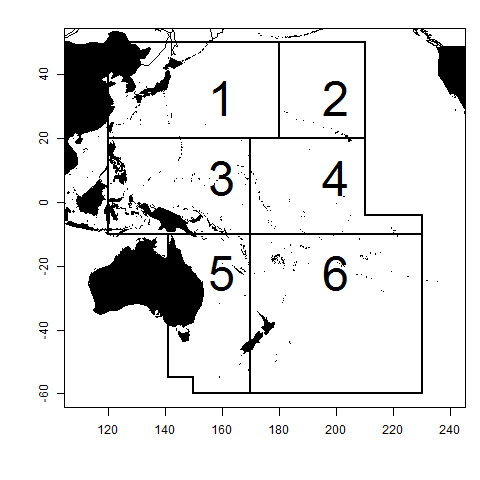
\includegraphics[width=\textwidth]{../GRAPHICS/Defined/FIG_01_MAP}
\caption{\label{fig:fig01} Map of the WCPO and regions used for the analysis.}
\end{center}
\end{figure}

%----------------------------------------------------------------------------------------

\subsection{Longline Fishery Data}
%---------------------------------------------------------------------------------------------
  
Longline fishing effort in the WCPO has increased steadily over the study period (1995-2014) to approximately 800 million hooks, with nearly half of the effort occurring in Regions 3 and 4 (Table \ref{tab:hooksfished}).  Ideally, indicator analyses would be based on operational-level data as its higher spatial resolution permits more comprehensive and nuanced analyses, however SPC’s operational level data are geographically limited and not consistent with the spatio-temporal distribution of the fleet.  Figure \ref{fig:fig02} illustrates the geographic distribution of longline logsheet data held by SPC (blue points). However, this picture is somewhat misleading as only 41\% of the sets plotted recorded sharks. This is in contrast to the observer data (orange points) in which 93% of the sets recorded at least one shark (red points).

This discrepancy is not necessarily due to misreporting. Prior to February 2011, sharks were not amongst the species for which data provision was required \citep{WCPFC2011_a}; since that time data provision for the 14 species designated by WCPFC as key shark species has been mandatory. Figure \ref{fig:fig02} does not distinguish between key shark species and other shark species because only 16\% of the reported sets recorded any species-specific shark catches. \citet{Clarke2011_b} note that most historical species-specific shark catch data are provided by a small number of flag States.

Given the relatively low level of coverage in the operational data, a more complete characterisation of the longline fishery requires the use of the aggregated (5\degree $\times$ 5\degree grid) data. Effort and reported shark catch by flag at the aggregated level have a lower degree of spatial resolution but in most cases are raised to represent the entire WCPO longline fishery. Sets with observers present onboard, are shown for comparison (Figure \ref{fig:fig03}) but have a finer degree of spatial resolution due to observer record keeping. 

A comparison of longline effort by flag and the number of sharks recorded in logsheets was constructed (Figure \ref{fig:fig04}) by showing the top four fishing nations (in the WCPO as a whole) and aggregating the rest of the flag states to another group. If the fishing practices and reporting practices were more or less consistent across flags the numbers of sharks reported would be proportional, by flag, to the effort.

Comprehensive data on shark catch at high spatial resolution are available from observer data held by the SPC-OFP but, as described above, the overall coverage of these data is low, and much less than the required levels of ROP coverage. In addition, a comparison of longline effort and longline observer coverage (Figure \ref{fig:fig05}) reveals that the latter is disproportional by region and flag and thus cannot be considered representative of the fishery as whole.

Due to the low data coverage, the observed sets are not spatio-temporarily representative of the fishing effort. A comparison of the number of sets observed by month - on a regional basis - shows significant fluctuations in the relative coverage of the observer data compared to the logbook data (Figure \ref{fig:fig06}).

Prior to all of the analyses performed in this report, the longline dataset was groomed according to the filters outlined in Table \ref{tbl:datfiltering}.

\begin{figure}
\begin{center}
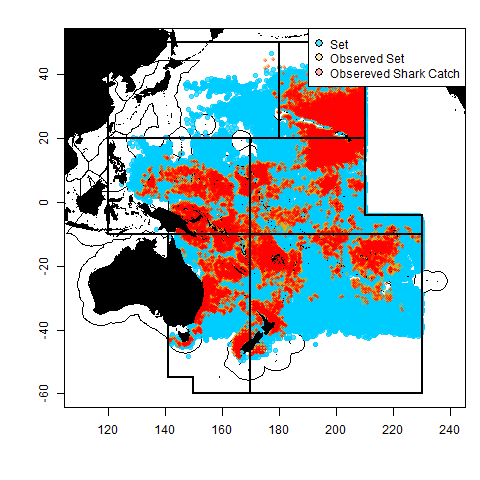
\includegraphics[scale=0.95]{../GRAPHICS/Defined/FIG_02_MAP_sets}
\caption{\label{fig:fig02} Reported sets (blue points), observed sets (orange points) and observed shark catch (red points) in the longline fisheries of the WCPO, from 1995-2014}
\end{center}
\end{figure}

\begin{figure}
\begin{center}
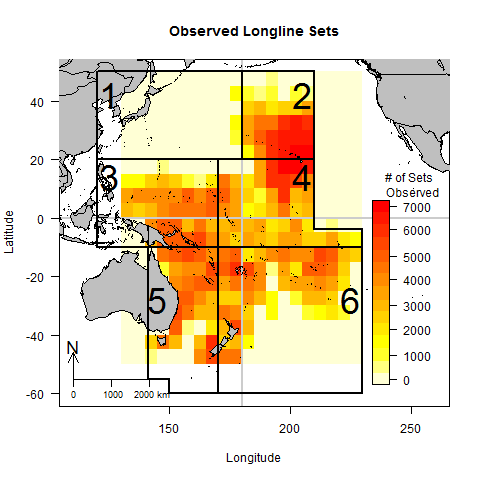
\includegraphics[scale=0.95]{../GRAPHICS/Defined/FIG_03_obs_ll_sets}
\caption{\label{fig:fig03} Longline observed sets by 5\degree $\times$ 5\degree square}
\end{center}
\end{figure}

\begin{landscape}
\begin{figure}
\centering
   \begin{subfigure}[b]{0.6\textwidth}
       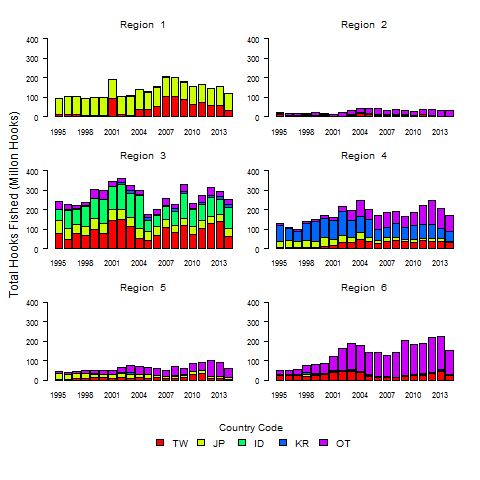
\includegraphics[width=\textwidth]{../GRAPHICS/Defined/FIG_04a_LLeff_FLAG_RDS}
       \caption{Longline effort.}
       \label{fig:fig04a}
   \end{subfigure}
   \begin{subfigure}[b]{0.6\textwidth}
       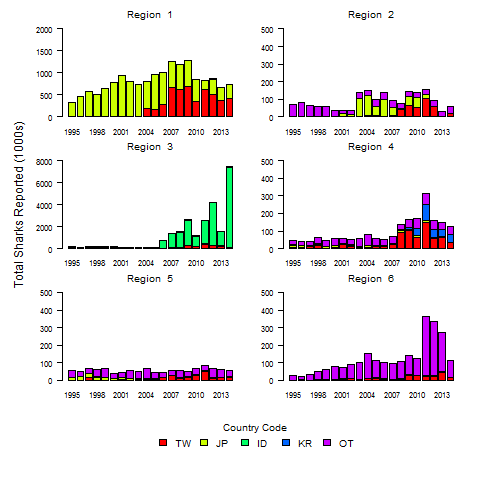
\includegraphics[width=\textwidth]{../GRAPHICS/Defined/FIG_04b_LLreported_catch_FLAG_RDS}
       \caption{Reported total shark catch.}
       \label{fig:fig04b}
   \end{subfigure}
\caption{Longline effort by flag and the number of sharks reported in logsheets}
\label{fig:fig04} 
\end{figure}
\end{landscape}

% FIGURE 5
%%%%%%%%%%%%%%%%%%%%%%%%%%%%%%%%%%%%%%%%%%%%%%%%%%%%%%%%%%%%%%
\begin{landscape}
\begin{figure}
\centering
   \begin{subfigure}[b]{0.6\textwidth}
       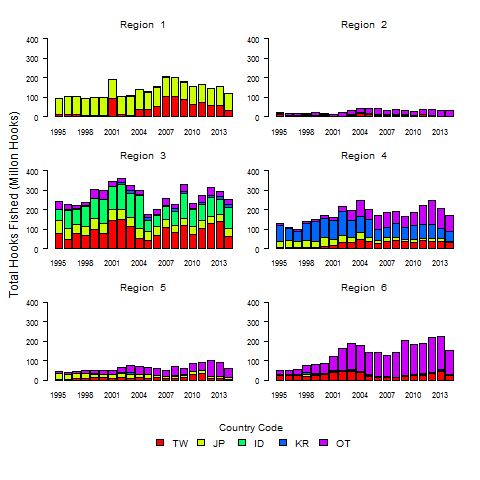
\includegraphics[width=\textwidth]{../GRAPHICS/Defined/FIG_05a_LLeff_FLAG_RDS}
       \caption{Longline effort.}
       \label{fig:fig05a}
   \end{subfigure}
   \begin{subfigure}[b]{0.6\textwidth}
       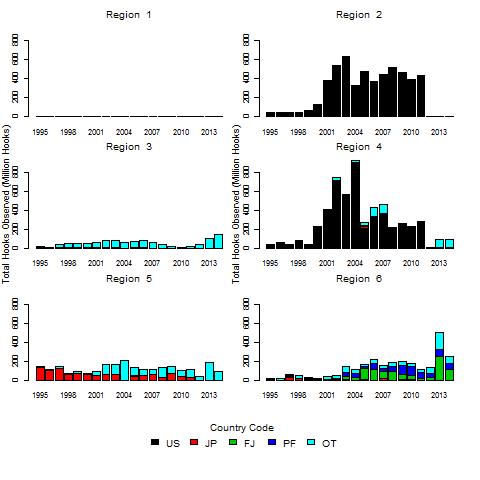
\includegraphics[width=\textwidth]{../GRAPHICS/Defined/FIG_05b_LLeff_obs_FLAG}
       \caption{Observer coverage.}
       \label{fig:fig05b}
   \end{subfigure}
\caption{Longline effort by flag and the extent of observer coverage}
\label{fig:fig05} 
\end{figure}
\end{landscape}
%%%%%%%%%%%%%%%%%%%%%%%%%%%%%%%%%%%%%%%%%%%%%%%%%%%%%%%%%%%%%%
% FIGURE 6
\begin{landscape}
\begin{figure}
\centering
   \begin{subfigure}[b]{0.6\textwidth}
       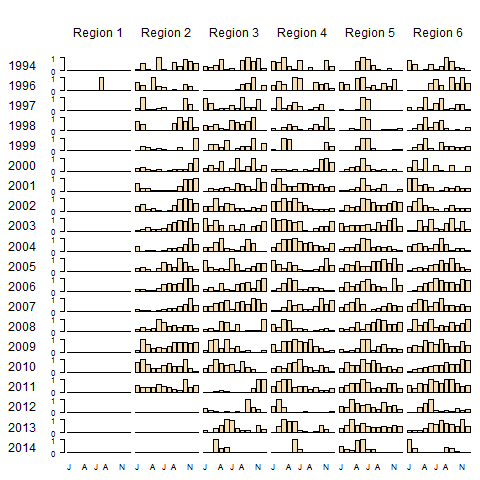
\includegraphics[width=\textwidth]{../GRAPHICS/Defined/FIG_06a_obsBY_mm_RDS}
       \caption{Longline effort.}
       \label{fig:fig06a}
   \end{subfigure}
   \begin{subfigure}[b]{0.6\textwidth}
       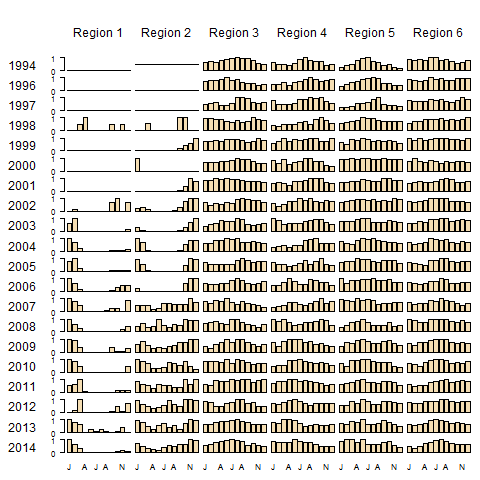
\includegraphics[width=\textwidth]{../GRAPHICS/Defined/FIG_06b_LOGSHEET_mm_RDS}
       \caption{Observer coverage.}
       \label{fig:fig06b}
   \end{subfigure}
\caption{Monthly breakdown of longline effort by region and the extent of observer coverage}
\label{fig:fig06} 
\end{figure}
\end{landscape}
%%%%%%%%%%%%%%%%%%%%%%%%%%%%%%%%%%%%%%%%%%%%%%%%%%%%%%%%%%%%%%
%\addcenterfig[Logsheet effort by month.]{fig:logeffmnth}{}
%\addcenterfig[Observed effort by month.]{fig:obseffmnth}{FIG_xx_obsBY_mm}
%\addcenterfig[Absolute percent difference in effort between reported (logsheet)  effort and observed effort.]{fig:effdiff}{FIG_xx_obsDIFFlog_mm}

\clearpage
%\addcenterfig[Aggregate effort by region. ]{fig:aggeff}{FIG_xx_agg_eff}
 
%-------------------------------------------------------------------------------------------------------------------------
 
 \subsection{Purse Seine data} 
 %N.B. all the stats quoted here are in PS_oper_stats.r (JR)
Similar to the longline fishery, SPC-OFP holds logsheet data on shark catch by purse seine fisheries at both the operational and aggregate levels.  However, operational-level coverage for the purse seine fishery (87\%) is considerably higher than for the longline fishery (23\%). This factor, in combination with the more limited geographic range of the purse seine fishery, contributes to more representative operation-level coverage in the purse seine fishery than in the longline fishery.

Following implementation of the WCPFC ROP on 1 January 2010, in combination with prior observer coverage commitments by Parties to the Nauru agreement (PNA) members, 100\% purse seine observer coverage is now required (except for vessels fishing exclusively in one Exclusive Economic Zone (EEZ)). Historical observer coverage in the purse seine fishery has varied between EEZs. Coverage rates were low, generally less than 10\%, for the years 1995-2002, with coverage increasing to 10-18\% for the years 2003-2009. Recent (2010-2013) annual averages are between 42-56\% in total.


While observer coverage of the purse seine fishery is not uniformly representative (Figure \ref{fig:fig07}, orange points), it is more representative than observer coverage of the longline fishery, owing to both higher coverage levels and the more limited geographic range of the fishery (Lawson 2011). Regions 3 and 4 contain 98\% of the operational-level reported purse seine sets, and 99\% of observed sets and are thus the only regions for which purse seine analyses will be meaningful. Shark interactions are recorded in just 2.5\% of purse-seine logsheets (Figure \ref{fig:fig07}, red points), a value far lower than the 41\% recorded in longline logsheet. As a result, it is not possible to assess the number of shark interactions by set or the species involved using purse seine logsheet data.

A comparison by flag of purse seine effort and the number of purse seine sets reporting at least one shark interaction was constructed for associated (Fish Aggregating Device [FAD]) and unassociated (free school) sets based on aggregated data (Figure \ref{fig:fig08}).  For each panel, flags were ranked by number of sets and the top four flags were plotted separately with all remaining flags aggregated into an "Other" category. Although estimated shark catch in the purse seine fishery are considerably lower than the longline fishery (SPC 2008, Lawson 2011), it would still be expected that purse seine shark interactions are proportional to purse seine effort. However, from the discrepancies between observed  and reported catch, it appears that some major fishing nations are not submitting or are under-reporting shark interactions.


%Figure 7
\begin{figure}
\begin{center}
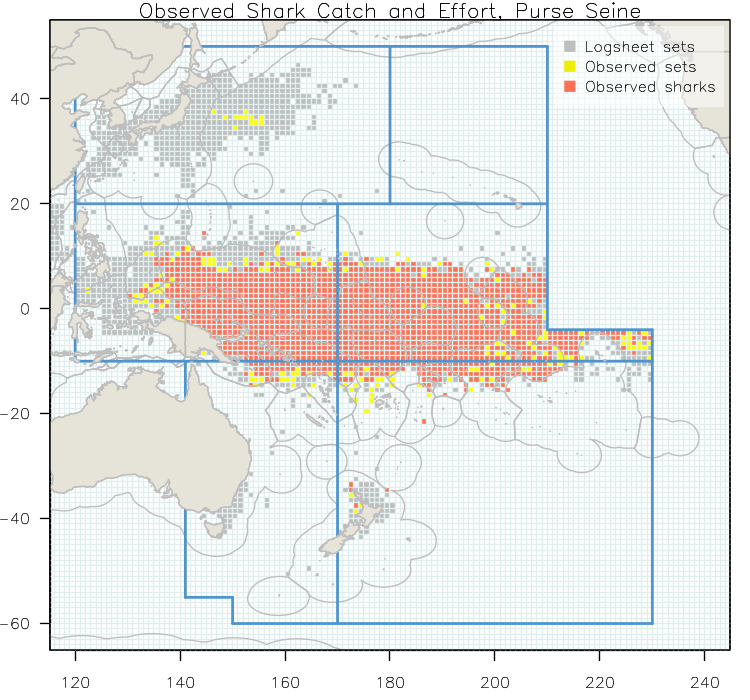
\includegraphics[scale=0.75]{../GRAPHICS/Defined/FIG_07_PS_sets}
\caption{\label{fig:fig07} Absolute percent difference in effort between reported (logsheet)  effort and observed effort.}
\end{center}
\end{figure}

% FIGURE 8
\begin{landscape}
\begin{figure}
\centering
   \begin{subfigure}[b]{0.49\textwidth}
       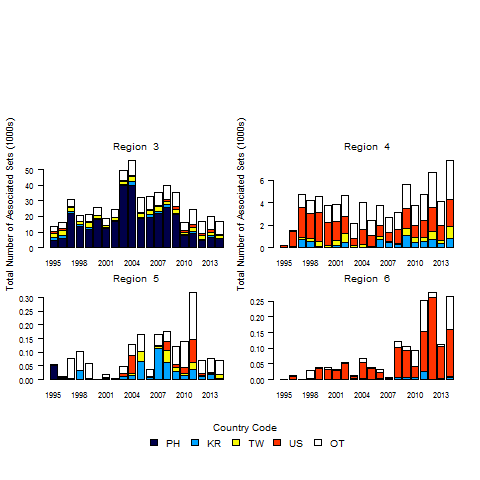
\includegraphics[width=\textwidth]{../GRAPHICS/Defined/FIG_08a_ps_total_effAssociated}
       \caption{Purse seine effort (Associated).}
       \label{fig:fig08a}
   \end{subfigure}
   \begin{subfigure}[b]{0.49\textwidth}
       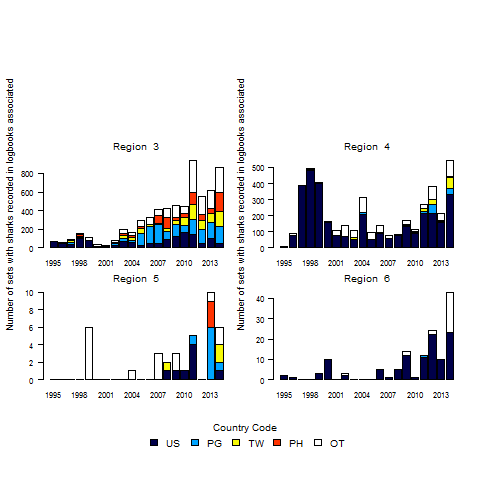
\includegraphics[width=\textwidth]{../GRAPHICS/Defined/FIG_08b_ps_oper_shks_rep_cntry_associated}
       \caption{sharks reported from associated sets.}
       \label{fig:fig08b}
   \end{subfigure}

   \begin{subfigure}[b]{0.49\textwidth}
       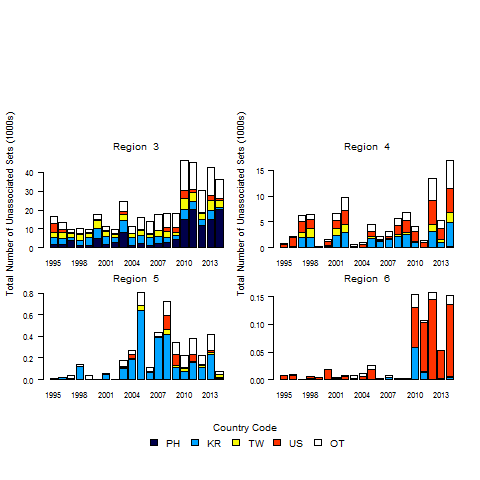
\includegraphics[width=\textwidth]{../GRAPHICS/Defined/FIG_08c_ps_total_effUnassociated}
       \caption{Purse seine effort (Unassociated).}
       \label{fig:fig08c}
   \end{subfigure}
   \begin{subfigure}[b]{0.49\textwidth}
       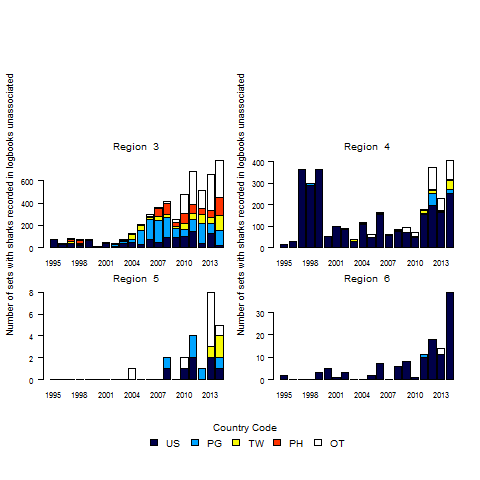
\includegraphics[width=\textwidth]{../GRAPHICS/Defined/FIG_08d_ps_oper_shks_rep_cntry_unassociated}
       \caption{Sharks reported from unassociated sets.}
       \label{fig:fig08d}
   \end{subfigure}
\caption{Purse seine effort by flag and the number of sharks reported for associated and unassociated sets.}
\label{fig:fig08} 
\end{figure}
\end{landscape}
        
%----------------------------------------------------------------------------------------
%  Distribution Indicators
%----------------------------------------------------------------------------------------
             
        
\section{Distribution Indicator Analyses}
      \subsection{Introduction}

      Distribution indicators consider patterns in the geographic distribution of catch. Spatial trends in fisheries data need to be interpreted carefully since they originate from biased design \citep{Walters2003_a}. If assessed carefully, however, they can provide useful insight into spatial and temporal trends in distribution as well as highlight areas of strong interactions between a species and fisheries. In addition, changes in stock abundance might be reflected in distribution\citep{MacCall1990}, with increases and decreases in abundance resulting in range expansions and contractions, respectively. Such patterns have been reviewed at length in the terrestrial literature (Borregaard et al., 2010), but less often for marine applications due to the paucity of historical data (but see Worm and Tittensor, 2011). The indicators presented below are based on observer data and thus patterns in fishing effort and/or observer coverage may bias the results.  These results should therefore be interpreted as potential indicative of the location and intensity of interactions between these species and WCPO longline fisheries.  These indicators can be updated over time to determine if the spatial patterns change or temporal trends change.  More complex methodologies might also be applied to remove potential sampling biases.
            
      \subsection{Methods}
      In this study, we calculated four Distribution Indicators:
      
\begin{itemize}
\item	Species-occurrence.  This indicator summarises the occurrence of a species in any longline set monitored by an observer.  A positive value at any given location simply indicates that the species in question was observed at least once, without regard to annual frequency or fishing effort.

\item	Proportion-presence.  This indicator provides a rough indicator of the frequency of occurrence of each species in each region and trends in presence over time.  Using observer data, the indicator is computed by dividing the total number of sets with at least one occurrence by the total number of sets in each region/year combination.
\item	High-CPUE.  This indicator is intended to illustrate which regions and years have shown relatively high CPUE values for the different species.  The index is constructed, again on the basis of observed longline sets, by computing mean CPUE within each 5\degree $\times$ 5\degree cell within each of the six regions, and then calculating the proportion of cells within a region that are above a specific threshold.  For this analysis, the threshold was set at 1 shark per 1000 hooks for blue shark and at 1 shark per 5000 hooks for the other species.
\item	Catch-Hotspot.  This indicator is an extension of the Species-occurrence and Proportion-presence indicators, and is intended to illustrate the possible presence of variable species catch hotspots.  All observed data are totalled within 1\degree $\times$ 1\degree cells over four separate five-year (pentad) periods.  The proportion of observed sets containing at least one species occurrence within that cell/pentad cell is then computed and mapped.  This provides better temporal resolution than the Species-occurrence indicator and better spatial resolution than the Proportion-presence indicator in helping to identify the distributional patterns of each shark species.
\end{itemize}



\subsection{Results}
The four sets of Distribution Indicators are grouped in Appendix B.1, as follows: Species occurrence (Figures \ref{IA_01} to \ref{IA_07}), Proportion-presence (Figure \ref{IA_08}), High-CPUE (Figure \ref{IA_09}), Hot spot analysis (Figures \ref{IA_10} to \ref{IA_16}).  Species-specific results below reference these sets of figures.
      
        \subsubsection{Blue Shark}
Blue sharks are the most common and widely reported shark species in WCPO longline fisheries.  They occur through the range of longline fishing and have the highest proportion-presence rate in virtually all years and regions among the shark species analysed there.  Both the Proportion-presence and High-CPUE time series show distinct downwards trends from the late 1990s to the present in most regions (3, 5, and 6).  Regions 2 and 4 show less distinct temporal trends.  The Catch-hotspot indicator shows consistently high occurrence of blue shark in longline fishery around the Hawaiian Islands with occurrence generally declining to the south, before again increasing in frequency around 20\degree{}S.


%----------------------------------------------------------------------------------------
\subsubsection{Mako Shark}
Mako sharks are one of the most commonly captured shark species in the longline fisheries of the WCPO.  Mako sharks have been encountered in longline sets in all regions that observers have sampled.  The largest, most consistent, hotspots have included waters in Region 5 between Australia and New Zealand.  Spatially, there are differing trends over time in the Proportion-presence and High-CPUE indicators.  The north and west regions (2 and 3) show stable or slightly increasing rates (though data for region 2 is lacking for years 2012-2014) whereas the south Regions (5 and 6) show steadily declining rates.

         
%----------------------------------------------------------------------------------------
 \subsubsection{Silky Shark}
 Silky sharks are commonly encountered in Regions 3 through 6 and at a very low rate in Region 2.  Neither the Proportion-presence nor High-CPUE indicators illustrate sustained temporal trends in occurrence.  The region with the greatest proportion of High-CPUE occurrence is Region 3.  The Catch Hotspot indicator also illustrates a consistency in both the temporal and spatial encounter of the longline fishery with silky sharks.
 %JR: For silky shark there seems to be a slight downward trend in the core regions of 3 and 4
%----------------------------------------------------------------------------------------
 \subsubsection{Oceanic Whitetip Shark}
 Oceanic whitetip sharks also occur with regular frequency in observed longline sets through most of the WCPO longline fisheries.  In the five regions where they are commonly encountered (Region 1 contains few observed sets) the trend in both Proportion-presence and High-CPUE has been declining steadily since the mid-1990s, with some of the decline in rates exceeding 80\%.  Catch-hotspots for oceanic whitetip sharks have been in the central Pacific, particular the region surrounding the junction of Regions 3, 4, 5, and 6.

%----------------------------------------------------------------------------------------
 \subsubsection{Thresher Shark}
 Thresher sharks have been found in observed longline sets in most regions of the WCPO with the possible exception of the area around French Polynesia. Catch-hotspots have been north of the equator, especially in Region 4. Both the Proportion-presence and High-CPUE time series show indistinct temporal trends though Regions 3 and 4 have dropped considerably over the past five years.

%----------------------------------------------------------------------------------------
 \subsubsection{Hammerhead Shark}
 Among the shark species analysed in this report, hammerhead sharks have the lowest encounter rates (measured as Proportion-presence) and appear to be patchily distributed.  The regions with the apparent largest presence of hammerhead sharks is the Northeast (Hawaiian Islands) and Southwest (Papua New Guinea, Australia east coast).  Due to the low encounter rates, little inference can be made regarding temporal trends in occurrence.
         
%----------------------------------------------------------------------------------------
 \subsubsection{Porbeagle Shark}
 Porbeagle sharks have historically only been encountered in the southern region of the WCPO, essentially only south of 20 \degree S (Regions 5 and 6).  A decrease in the spatial and temporal occurrence of porbeagle in observed sets is evident in the three Distribution Indicators other than Species-occurrence.  The porbeagle catch-hotspots have shrunk both in size and intensity over the four pentads; the Proportion-presence and High-CPUE time series for Regions 5 and 6 have declined as much as 90\% over the past 15 years.
 
     
          
  \subsection{Conclusions}
  
The Species occurrence indicators show that all seven species examined here, with the exception of porbeagle and hammerheads, are encountered across the breadth of the WCPFC region; hammerheads are distributed more patchily while porbeagle are restricted to the region south of 20\degree{}S. With the exception of blue shark and oceanic whitetips, the Proportion-presence and High-CPUE indicators showed a more or less steady trends for all species in all regions.  for those two species, both indicators have shown declines as great as 80\% in Regions 3 through 6.  
  
Interpretation of the distribution indicators, particularly the Catch-Hotspot indicators, is complicated by the influence of changes in fishing effort,  potential  changes in community composition, observational coverage  and operational factors influencing selectivity and catchability (e.g. depth and leader material). As such, these indicators are best used for identifying the areas in which species-fishery interactions take place, and as supporting information for interpreting other patterns and trends. 
% Distribuion Indicators 

%----------------------------------------------------------------------------------------
%  Species Composition
%----------------------------------------------------------------------------------------
      
      
\section{Observed Species Composition Indicator Analyses}

 \subsection{Introduction}
Changes in the species composition of the catch can be one of the most direct indicators of fishing induced changes to fish assemblages over time. Additional information on potential changes can be inferred by examining catch data on a finer basis, e.g., by separating longline sets by depth and purse seine sets by type of school association. We rely on observer sampling of individual sets for such analyses. Additionally, by examining time series of catch composition we can ascertain whether there has been a decline in the percentage of unidentified sharks; improvements in observers’ ability to identify sharks to the species level can help resolve or identify potential regional and temporal trends in abundance.

We compile the observer data to provide information on the relative proportion of key species in observer sample. Nevertheless, it is an ongoing issue that observer sampling may not be representative of total catch composition due to issues of uneven coverage and low sample sizes. Those issues are covered in detail in Lawson (2011). However, these data represent the best that we have and temporal/spatial changes in relative species composition can help identify population increases or decreases. More direct species-specific analyses, such as summarised in section 5, should be performed to assess the veracity of identified abundance changes.

Species Composition Indicator Figures are illustrated in Appendix B.2 for longline (Figures \ref{SC_01} to \ref{SC_03}) and purse seine (Figures \ref{SC_04} to \ref{SC_06})

      
  \subsubsection{Longline}  
  

With just a few exceptions, blue shark catch dominates the longline shark bycatch.  In Regions 2, 4, 5, and 6, blue sharks have average 60-90\% of shark bycatch; in Region 4 the proportion of blue shark has dropped from around 60\% in the late 1990s to 10-15\% in recent years.  The second most common observation of shark species, in terms of numbers, is silky shark which have constituted a majority of shark bycatch in Region 3 since the early 2000s and have been on the order of 5-10\% in other regions.  We note that there appears to be a sudden increase in the proportion of silky shark catch for Region 4 in years 2012-2104.  This reflects the absence of observer data from the U.S. longline fleet operating around Hawaii rather than a chance in speceis composition.  As evidenced by the small number of observed sets shown for years 2012-2014, the shark composition data for these years in Region 4 are quite likely unrepresentative.  Several of the other key shark species constitute up to 10\% of the shark bycatch in certain regions and time periods: porbeagle in Regions 5 and 6, oceanic white tip sharks in Regions 3, 4, and 6 and thresher sharks in regions 3 and 4.  The other, or non-key species, observed in Regions 5 and 6 were primarily composed of roughskin dogfish (Centroscymnus owstoni) and tope shark (Galeorhinus galeus), and in Region 3 were primarily composed of unidentified hammerhead, grey reef (Carcharhinus amblyrhynchos) and blacktip (Carcharhinus limbatus) sharks. Unidentified sharks comprised no more than 1.6\% of the recorded sharks in any of the regions.

Division of the longline shark bycatch into shallow ($<$11 hooks per basket) and deep ($>=$11 hooks per basket) sets revealed several differences in the assemblage of sharks caught at depth.  Regions 3, 5, and 6 each have relatively large number of observed sets so we restrict our comparison to those Regions.  In the southern Regions (5 and 6), blue shark and porbeagle comprise as much as 95\% of the longline shark catch; the deep water sets contain a much more diverse array of species with silky, thresher, oceanic whitetip and mako sharks occurring in substantial numbers.  Differences in shark composition in Region 3 are much more subtle than Regions 5 and 6; hammerhead and oceanic white tip sharks are more common in deep sets while silky sharks are a bit more common in shallow sets. There was no strong indication of temporal trends specific to deep or shallow sets.

  
%------------------------------------------------------------------------------------------
 \subsubsection{Purse Seine} 
The majority of purse seine caught sharks have been identified to species in observer samples since the late 1990s.  Prior to that, it is likely that practical difficulties, such as sharks not being hauled aboard, resulted in non-identification.  Sample sizes were small during that time period making it difficult to generalize trends before 2000.  Overall, silky shark comprise at least 70\%, and often more than 90\%, of the sharks captured in purse seine sets; both in associated and unassociated sets.  Oceanic whitetip and hammerhead sharks have also been caught in notable.

 
\subsection{Conclusions}

The Species Composition indicators reveal that shark bycatch differs substantially between longline and purse seine fishing in the WCPO.  

Blue sharks are the most prevalent longline caught shark, but there are substantial regional and depth variations.  Several species are commonly caught more frequently in deeper sets; porbeagle form a sizeable component of the shallow sets in the regions where they occur (i.e., Regions 5 and 6) and silky shark is the second most common longline caught shark.

Purse seine shark bycatch is much less specious and is dominated by silky sharks, particularly over the past decade when the number of observed sets increased greatly and composition data may have become more representative.  In virtually all regions and years, silky shark comprises more than 95\% of the shark bycatch, with minor numbers of hammerhead and oceanic whitetip sharks occurring.  Oceanic white tip sharks appear to have been more common prior to 2000, their percentage contribution to the overall shark catch has not been more than 20\% in regions 3 and 4 for over a decade, which is stark contrast to the first ten years of the study period. 

 \clearpage          

%----------------------------------------------------------------------------------------
%  CPUE INDICATORS
%----------------------------------------------------------------------------------------
\section{Catch Per Unit Effort indicator analyses}

%\documentclass{SCreport}

%\begin{document}
%%%%%%%%% Defining latex macros to print tables %%%%%%%%%%


\newcommand{\blueaic}{
% latex table generated in R 3.2.0 by xtable 1.7-4 package
% Sat Jul 04 14:52:03 2015
\begin{table}[ht]
\centering
\caption{AIC improvement over null model for blue from a single explanatory variable} 
\label{blue:aic1}
\begin{tabular}{lrr}
  \hline
Variable & AIC.diff & AIC.diff.sigma \\ 
  \hline
program\_code & 24382.47 & 16607.68 \\ 
  flag\_id & 23711.29 & 17163.94 \\ 
  HPBCAT2 & 20183.28 & 5765.59 \\ 
  HPBCAT & 20178.74 & 5576.42 \\ 
  yy & 14357.75 & 8612.54 \\ 
  mm & 3725.06 & 2511.55 \\ 
  sharkbait & 994.97 & 454.07 \\ 
   \hline
\end{tabular}
\end{table}

}


\newcommand{\makonorthaic}{
% latex table generated in R 3.2.0 by xtable 1.7-4 package
% Sat Jul 04 14:52:03 2015
\begin{table}[ht]
\centering
\caption{AIC improvement over null model for mako.north from a single explanatory variable} 
\label{mako.north:aic1}
\begin{tabular}{lrr}
  \hline
Variable & AIC.diff & AIC.diff.sigma \\ 
  \hline
HPBCAT2 & 6433.14 & 642.33 \\ 
  HPBCAT & 6417.24 & 640.61 \\ 
  mm & 2845.80 & 216.50 \\ 
  yy & 2216.05 & 401.91 \\ 
  flag\_id & 115.74 & 61.51 \\ 
  program\_code & 114.17 & 44.28 \\ 
  sharkbait & 15.46 & 3.29 \\ 
   \hline
\end{tabular}
\end{table}

}


\newcommand{\makosouthaic}{
% latex table generated in R 3.2.0 by xtable 1.7-4 package
% Sat Jul 04 14:52:03 2015
\begin{table}[ht]
\centering
\caption{AIC improvement over null model for mako.south from a single explanatory variable} 
\label{mako.south:aic1}
\begin{tabular}{lrl}
  \hline
Variable & AIC.diff & AIC.diff.sigma \\ 
  \hline
program\_code & 1693.97 & 251.6 \\ 
  flag\_id & 1438.39 & --- \\ 
  HPBCAT2 & 1202.23 & 79.45 \\ 
  HPBCAT & 1127.42 & 34.67 \\ 
  yy & 875.66 & 389.5 \\ 
  mm & 733.11 & 178.28 \\ 
  sharkbait & 8.37 & -1.89 \\ 
   \hline
\end{tabular}
\end{table}

}


\newcommand{\ocsaic}{
% latex table generated in R 3.2.0 by xtable 1.7-4 package
% Sat Jul 04 14:52:03 2015
\begin{table}[ht]
\centering
\caption{AIC improvement over null model for ocs from a single explanatory variable} 
\label{ocs:aic1}
\begin{tabular}{lrr}
  \hline
Variable & AIC.diff & AIC.diff.sigma \\ 
  \hline
yy & 3726.21 & 958.91 \\ 
  program\_code & 2781.62 & 1369.09 \\ 
  flag\_id & 1499.89 & 772.13 \\ 
  sharkbait & 887.50 & 103.91 \\ 
  HPBCAT2 & 308.22 & 1656.57 \\ 
  HPBCAT & 256.09 & 1658.57 \\ 
  mm & 143.92 & 185.56 \\ 
   \hline
\end{tabular}
\end{table}

}


\newcommand{\silkyaic}{
% latex table generated in R 3.2.0 by xtable 1.7-4 package
% Sat Jul 04 14:52:03 2015
\begin{table}[ht]
\centering
\caption{AIC improvement over null model for silky from a single explanatory variable} 
\label{silky:aic1}
\begin{tabular}{lrr}
  \hline
Variable & AIC.diff & AIC.diff.sigma \\ 
  \hline
program\_code & 10913.31 & 6886.75 \\ 
  flag\_id & 10144.24 & 5446.47 \\ 
  sharkbait & 5382.46 & 1713.24 \\ 
  yy & 4986.96 & 3273.31 \\ 
  HPBCAT2 & 1639.75 & 4527.65 \\ 
  HPBCAT & 1628.44 & 4513.75 \\ 
  mm & 957.50 & 358.96 \\ 
   \hline
\end{tabular}
\end{table}

}



\subsection{Introduction}

%This paper follows from the previous indicator based analysis presented to the Western and Central Pacific Fisheries Commission (WCPFC) Scientific Committee (SC7, Clarke et al. 2011), stock assements (Rice et al. 2014, Rice et al.2013, Rice et al.2012) \hllb{(cite the standardization papers, cite ISC work?)}. The developments presented here include additional analyses of the Secretariat of the Pacific (SPC) data holdings for silky caught in longline and purse seine fisheries in the Western and Central Pacific Ocean (WCPO), though we note that some previous data (Japan) was not available for this effort. Standardized catch per unit of effort (CPUE) series are developed for the main shark species.  
%\emph{Note: The current analysis does not construct inputs to use for stock assessments or catch estimates. Our goal is to highlight general trends in population abundance over time, to be interpreted together with other indicators as outlined above. We recommend that catch rates standardization for stock assessments or catch estimates be conducted independently.}


% intro      
Catch-per-unit-effort (CPUE) data are commonly used as indices of abundance for marine species. However, multiple factors---fishing technique, season, bait type, etc---can alter the relationship between CPUE and abundance, especially in complex fisheries systems comprising of several fleets and spanning large spatial and temporal scales. Nominal catch rates must therefore be standardized to account for changes in these factors over time. This is typically done using General Linear Models (GLM), which allow us to model the relationship between CPUE and a set of explanatory variables. The dataset used in this analysis provided many candidate variables, but, given the diversity of observer programs represented, few had enough coverage to be retained in the final models. The available variables are described in Table \ref{tbl:glm-vars} (see also Table 2 in \citet{Francis2014_b} for an overview of the use of variables in shark CPUE standardisations).

% issue with sharks cpue standrz
CPUE data for sharks often have a large proportion of observations (sets) with zero shark catch, while while some sets have large catch. These instances of high catch can occur when areas of high shark densities are accidentally encountered or when fishers target sharks. The co-existence of both high proportions of zeros and high catch results in over-dispersed data, typical of bycatch species. These features are challenging to account for from a statistical point of view, and have been reviewed at length in the literature on bycatch analyses \citep{Bigelow2002_a,Campbell2004_a,Ward2005_a,Minami2007_a}. 
%(Bigelow et al. 2002; Campbell 2004, Ward and Myers 2005; Minami et al. 2007).

Zero-inflated approaches have been advocated as best suited to model over-dispersion in both zeros and positive counts (Brodziak et al., 2013). A drawback of the zero inflated approach is that it is data intensive and models fail to converge. In addition, in practice it tends to be more successful at modelling the extra zeroes than the large-catch events, since the dispersion parameter which controls the length of the tail is assumed to be constant over all factors. This is especially a problem when the mean of the distribution is close to zero or one, as in those instances the probability of getting large events if mostly controlled by the dispersion parameter $\sigma$, unlike when the mean is larger and the tail is not as pronounced. However, whenever conditions are good for sharks and/or targeting takes place, larger catch events can happen and not modelling those properly implies that we are missing important drivers of catch. Typically, this can be diagnosed as a departure from the one-to-one line on the right-hand side of quantile-quantile plots. Here we achieved significant improvements in model diagnostics by keeping a negative binomial distribution but allowing both the mean $\mu$ and $\sigma$ parameters to be modelled against covariates \citep{Rigby2005_a}. This approach is much less computationally intensive than zero-inflated models, and yielded excellent diagnostics with these data.


 \subsection{Methods}
Standardised CPUE series for the longline bycatch fisheries were developed using generalised linear models using longline catch and effort data. The number of hooks in a longline set was used as a measure of effort.
See also \citet{Clarke2011_a, Clarke2011_b},  \citet{Walsh2011_a}, \citet{Rice2012_a}   for past work on shark CPUE standardisation in the Western and Central Pacific Ocean (WCPO).
%  @Article{,
 %   title = {Generalized additive models for location, scale and shape,(with discussion)},
 %   journal = {Applied Statistics},
 %   volume = {54},
 %   part = {3},
 %   pages = {507-554},
 %   year = {2005},
 %   author = {R. A. Rigby and D. M. Stasinopoulos},
 % }
 \label{cpuemeth:datafilter}
 \subsubsection{Stock definition for the purpose of the analysis}
   
% talk about stocks and year span                                                                                        
%Silky and oceanic white tip sharks are observed mainly in the equatorial waters in the purse seine fishery (Figure \ref{...}), and from about -25\degree~S to 25\degree~N in the longline fishery (Figure 1). 
Silky and oceanic whitetip sharks have each been assessed \citep{Rice2012_a, Rice2013_a} as single stocks in the WCPO, and are presented in this analysis as a single stock.  Thresher, mako and blue sharks occur more frequently in cold, temperate waters, and generally believed to be separated into northern and southern stocks. For instance, blue sharks in the North Pacific have been subject to multiple stock assessments as a stock unit. These temperate species are thus analysed as individual stocks. In the Pacific porbeagle sharks are only found south of 20\degree{}S and were analysed as a single stock. Hammerhead sharks for the purpose of this analysis (and throughout the report) are considered to be a single stock.

\subsubsection{Data Preparation}
To further define the expected geographic range, we defined a coarse climate `envelope' based on sea surface temperature. This aided in distinguishing between zero catch in areas where the species does not occur from zero catch in areas where the species occurs but was not caught. Temperature data were downloaded from the GODAS database (\url{www.cdc.noaa.gov/data/gridded/data.godas.html}) and matched to the observer data on a set by set basis. The temperature range of a species was defined as the minimum and maximum of the monthly mean sea surface temperatures (SST) of cells with positive catch for that species (see Table \ref{meth:temprange}). The temperature predicted by GODAS at the 5 meters depth at set time/day was used for the SST value. Only cells for which all mean monthly temperatures fell within this range were retained. %\hllb{REWORK. Note that this is a minimal filter and it was only used to exclude the most improbable cells from which a species could be seen.}
 %\hl{Looked at range of SST where positive catches occured, selected cells where median falls within this range.}
 
%                                                                        section \ref{app:datacleaning}     
          
Data were cleaned following the filters outlined in Table \ref{tbl:datfiltering}. Records from the US observer programs (Hawaii and American Samoa) were excluded from the analysis as they were only available up to 2011. Records from any observer programs for which we had less than 100 sets were removed. Extreme catch events greater than the $97.5^{th}$ quantile of the nominal CPUE were also removed. Finally, year effects were only estimated if there were at least 50 sets observed in that year (by species and population).  Records from the Papua New Guinea observer program were removed as vessels in the fleet frequently target sharks. Additional filters are listed by species in Table \ref{tbl:glmdata}.
                                                                                      
%Previous work \citep{Rice2012_a, Rice2013_a, Bromhead2012_a} has examined the extent of shark targeting in the WCPO tuna longline %fleet, and found that a number of factors (i.e. sharklines, wire trace can lead to a higher catch rates). Shark target sets comprise a much smaller proportion of the overall dataset (6.5\% of the sets), however, these sets represent significant shark catch for some species (e.g. 82\% of the total silky shark catch). Sets marked by observers as targeting sharks were therefore removed from the analysis as catch rates therein behave differently than when sharks are caught as by-catch. 
%Shark targeting sets were deemed to be sets where the observer had marked that the set was intentionally targeting sharks of any species, whether shark bait was used, or whether shark lines were used. We also removed the data from the Papua New Guinea observer program because of frequent shark targeting which may not always appear in observer records. 
                                                                                       
% \subsection{Additional categorical variables}    % jr edits don't think we need that
% 1. Day category: sunset and sunrise were calculated\\ 
% 2. HPBCAT: based on data exploration two types explored: either shallow or deep (with shallow $<=$ 10), or HPBCAT2 shallow, intermediate and deep, with intermediate between 10 and 15 ... in general hpbcat2 had slighlty better aic %(in tables at the end)
     %Latitude and longitude were truncated to the nearest 1\degree; this location information was used to calculate the set specific association with a 5\degree square (referred to hereinafter as cell). Date of set was used to calculate the year, month, quarter and trimester of the set. Set time was used to calculate the time category of the day in sixths starting at midnight. A non-target data set was created as a result of filtering data sets according to the above rules as well as filtering sets where sharks were the intentional target. This was done under the premise that the factors leading to non-zero catch rates when targeting sharks would be different than factors that lead to non-zero catch rates when not targeting sharks. 
                                                                                       
                                                                                       
   \subsection{Overview of GLM Analyses}
   \subsubsection{Notes on error distributions:} 
  
   The  filtered datasets  were standardised using generalized linear models \citep{McCullagh1989_a} with the software package R (\url{www.r-project.org}, \citealt{RCT2013_a}) and the package \texttt{gamlss} \citep{Rigby2005_a}. Initially, multiple assumed error structures were tested including the delta lognormal approach (DLN)   \cite{Lo1992_a, Dick2006_a, Stefansson1996_a}, zero-inflated poisson and negative binomial models, the tweedie distribution \citep{Shono2008_a} and negative binomial models with mu and  $\sigma$ modelled. Due to its superior performance both in run time and model diagnostics, we retained the latter and only present those results here.
%  in JR_bib_edts.bak Hiroshi Shono 2008. Application of the Tweedie distribution to zero-catch data in CPUE analysis. Fisheries Research 93 (2008) 154-162

%The negative binomial (Lawless, 1987) is typically more robust to issues of over-dispersion (over-dispersion can arise due to excess zeros, clustering of observations, or from correlations between observations) was also used. This model has been advocated as a model that is more robust to over-dispersion than the Poisson distribution (McCullagh and Nelder 1991), and is appropriate for count data (Ward and Myers  2005), but does not expressly relate covariates to the occurrence of excess zeros (Minami et al. 2007).
                                                                                       
 %    	Mixture models such the zero inflated Poisson (ZIP) and zero inflated negative binomial (ZINB) (Zuur 2009, Cunningham and Lindenmayer 2005, Welsh et al. 2000): these models are useful for modelling counts of rare species when the number of zero observations is larger than expected. Zero inflated models are a process similar to the delta approach in which the presence or absence of the catch is modelled orthogonally to the size of the catch (Welsh et al 2000), however unlike the delta approach the count data can include zeros. These zeros could result from predator satiation, competition for hooks, or disinterest (called true zeros) as opposed to design errors, sampling errors, observer errors or zeros resulting from sampling outside the habitat range (called false zeros). The total probability of a zero count is then,
\subsubsection{Procedure for model selection}
% cite AIC?Akaike, H. (1974), "A new look at the statistical model identification" (PDF), IEEE Transactions on Automatic Control 19 (6): 716-723, doi:10.1109/TAC.1974.1100705, MR 0423716.  get the table refs right 
Initial model exploration began via fitting each model (species and population) with only one covariate and evaluating the explanatory power of that covariate \via AIC (AIC values are listed in tables  listed in Tables~\ref{BSH.north:aic1} to \ref{THR:aic1}. Model fitting proceeded by fitting additional covariates in order of the proportion of deviance explained  on their own.  Only those covariates showing a change in AIC of 10 or greater were kept in the model.
%-- added covariate on MU ONLY (mean) until AIC showed decline $<$ 10 (arbitrary....) \\

If model diagnostics indicated a departure from the assumed error structure, covariates were added to $\sigma$ until the model mis-specification was resolved. Covariates were added based on the principle of a minimally efficient design and beginning with those covariates for which the AIC~$\sigma$ table (Tables \ref{BSH.north:aic1} to \ref{THR:aic1}) indicated had the most explanatory power.  

The addition of explicitly modelling the $\sigma$ greatly improved the  model diagnostics in  most cases where the Q-Q norm plot indicated a misspecification in the tail of the assumed distribution.  The objective of the CPUE standardisations were to produce CPUE values that accounted for changes in catch rate not due to changes in abundance over time, in this case the time step was an annual time step, therefore year effects were included in each model. 
All models also included either flag or observer program code, because flag and observer program are often highly correlated, one or the other as an explanatory categorical variable, based on the proportion of variance it explained and whether model diagnostics were impacted.
Interaction between year and observer program was also modeled in part to account for potential changes in individual program practices (e.g. reporting to species, banning shark fishing) within a particular program.  Additionally modelling year and program may account for localised trends in annual abundance, or sampling effort that are reflected in the program specific observer data. Other interaction effects were investigated early in the model selection process but discarded due to low explanatory power.%
% did I get this right?
%\hlgreen{but did not proceeded with an interaction for the remaining of the model selection}.
% huh? 
%as doing so would entail if the AIC
%score when interactions are allowed is at least 50 lower than with
%additive effects only.
                                                                                    
\subsubsection{Model diagnostics}                                                                                      
Model selection included examination of diagnostics including quantile residuals \citep{Dunn1996_a}, normal quantile-quantile plots, plots of the residuals residuals vs fitted factors, residuals vs. explanatory factors as well as an overall summary.
The quality of model fit was assessed by inspecting the residuals as well as simulating data from the fitted GLM model and comparing the simulated to the observed. Quantile residuals  were used instead of the traditional deviance or Pearson’s residuals. Quantile residuals overcome many of the problems encountered for count-based GLMs and greatly facilitate model diagnostics. Specifically we aimed to improve fit to both the zeros and high catch events. Diagnostics were satisfactory for all stocks except that of blue shark in the south Pacific for which high catch events were still not well modelled, presumably due to unaccounted targeting by some fleets. Key diagnostics are included in Figures \ref{fig:diagno1} to \ref{fig:diagno2}.


\subsubsection{Calculation of year indices and confidence intervals}
Year effects could be extracted directly from the model output as there were no interactions between year and other variables, and year was not included as an explanatory variable for the $\sigma$ models. Confidence intervals were computed with the function \texttt{confint} in the R package \texttt{stats}.
%Multiple methods of calculating the indices of abundance and confidence intervals exist depending on the model type (Shono H. 2008, Maunder and Punt 2004). In this study estimates were %calculated by predicting results based on the fitted model and a training data set that included each year effect and  the mean effect for each covariate (Zuur et al 2009). Confidence %intervals were calculated as ?1.96* SE, where SE is the standard error associated with the predicted year effect term.  Appendices hold the model diagnostics.
%%%%%
\clearpage
\subsection{Results}
%----------------------------------------------------------------------------------------

Nominal CPUE by species and region for longline sets are shown in Figures \ref{fig:nomCPUE} and \ref{fig:nomCPUErel} and for associated and unassociated purse seine sets in regions 3 and 4 in Figures \ref{fig:nomCPUEpsAss} and \ref{fig:nomCPUEpsUnass} respectively. Plots of nominal and standardised CPUE on a species by species basis are shown in Figures \ref{fig:blueStdCPUEnorth} to \ref{fig:thresherStdCPUE}.
 
\begin{description}
\item[Blue shark (\emph{Prionace glauca}), north Pacific] Both the standardised and nominal CPUEs of blue shark in the north Pacific show a declining trend starting in 1999 and 1998, respectively. Data points for 2011 and 2012 are unavailable due to low sample size.  
 
 \item[Blue shark (\emph{Prionace glauca}), south Pacific]  Both the standardised and nominal CPUEs for blue shark in the south Pacific show declines in the initial 1995-2003 and late 2010-2015 periods, with relatively stable CPUEs between 2004  and 2009.  
 
 \item[Mako shark complex (\emph{Isurus oxyrinchus} and \emph{I. paucus}) in the north Pacific] The standardised and nominal CPUEs share the same trajectories (Figure \ref{fig:makoStdCPUEnorth}), but on a slightly different scale for the first 6 years (1995-2001).  The largest difference in the nominal and standardised CPUE is in the final year, where the standardised CPUE declines sharply in contrast to the nominal, but years 2011 and 2012 were excluded from the standardisation due to poor sample sizes (Figure \ref{makoStdCPUEvars2}).
 
\item[Mako shark complex (\emph{Isurus oxyrinchus} and \emph{I. paucus}) in the south Pacific] The standardised CPUEs show a more stable trend in relative abundance than the nominal CPUEs, although both have low points in 2002 and 2014. In addition, the standardised CPUE peaks in 2010, whereas the nominal is the highest in 1996.
 
\item[Oceanic whitetip shark (\emph{Carcharhinus longimanus})] The standardised oceanic whitetip shark trend decreases steadily over 1995-2014.  The standardised trend shows a slightly steeper decline than the nominal, with the most noticeable departure from the nominal being the large decrease from 2013-2014 in the standardized CPUE.%   Diagnostics indicate no departure from the normality assumptions made in the mode.
 
 \item[Silky shark (\emph{Carcharhinus falciformis})] Standardised silky shark trends in the WCPO showed high inter-annual variability with an initial decline from 1995-2000 followed by a slight increase until 2010, followed by a steep decline. This mirrors the trends seen in the nominal CPUE, albeit with a lesser variability.
 
\item[ Thresher shark complex (\emph{ Alopias superciliousus, A. vulpinus, \& A. pelagicus})]  Standardised CPUE values for thresher sharks were similar to the nominal CPUE except for additional variability in the nominals. They both rise for the first 6 years of the series (1995-2001) but diverge thereafter. For 2002-2014, the standardised CPUE is less variable, decreasing slightly from 2003-2011. The last three years of both the standardised and nominal CPUEs show a steep decline.  The CPUE from the thresher complex is difficult to interpret as the second most commonly reported thresher species is the general ``thresher shark" category. 
 
\item[Hammerhead shark complex (\emph{ Sphyrna mokarran, S. lewini, S. zygaena, \& Eusphyra blochii})]  Standardised CPUE for the hammerhead complex shows a large increase from the 3rd to the 6th year of the study period (1997-2001), with a relatively stable CPUE thereafter (2002-2013, regions 3 and 5 in the longline database). Similar to the thresher shark complex, the CPUE series representing the hammerhead complex are difficult to interpret because more than half of the observations in the study period (1995-2014) were recorded into the generic ``hammerhead'' category.
 
 \item[Porbeagle shark (\emph{ Lamna nasus}) ] The standardised CPUE for porbeagle shark was close quite similar to the nominal CPUE, showing an increase in the first three years of the time series, followed by a decline from 1999 to 2003, and a monotonic increase thereafter.
 
 
%\item[ Whale Shark (\emph{ Rhincodon typus}) ] Whale shark interactions are generally reported only by the purse seine fishery. These observations are subject to considerable spatial and temporal heterogeneity and likely to have been affected by changes in observer coverage and reporting practices in recent years. The fate of whale sharks following interactions is also uncertain and information on key biological processes are limited. Given the current SPC data holdings only limited analysis for whale sharks in the WCPO is considered to be feasible.
 
\end{description}

%\addcenterfig[Blue shark CPUE indicators. Proportion of positive sets, observer data.]{fig:bshcp1}{FIG_xx_pcntpos_reg_BSH}
%\addcenterfig[Blue shark CPUE indicators. Nominal CPUE, sharks per 1000 hooks, observer data.]{fig:bshcp2}{FIG_xx_nomCPUE_reg_BSH}
%\addcenterfig[Blue shark CPUE indicators. Standardized blue shark CPUE based on the negative binomial model for observer data in the northern hemisphere.]{fig:bshcp3}{LLcpue_BSH_north_NB_step}
%\addcenterfig[Blue shark CPUE indicators. Standardized CPUE, zero inflated negative binomial Southern Hemisphere, observer data.]{fig:bshcp4}{ll_cpue_BSHzinb_nominal}

%----------------------------------------------------------------------------------------
          
%\addcenterfig[Mako shark CPUE indicators. Proportion of positive sets, observer data.]{fig:makcp1}{FIG_xx_pcntpos_reg_MAK}
%\addcenterfig[Mako shark CPUE indicators. Nominal CPUE, sharks per 1000 hooks, observer data.]{fig:makcp2}{FIG_xx_nomCPUE_reg_MAK}

%\addcenterfig[Mako shark CPUE indicators. Standardized CPUE, mako shark in the northern hemisphere.]{fig:makcp3}{LLcpue_MAKO_north_NB_cpue}
%\addcenterfig[Mako shark CPUE indicators. Standardized CPUE, mako shark in the southern hemisphere.]{fig:makcp4}{LLcpue_MAKO_south_NB_cpue}

%----------------------------------------------------------------------------------------

%\addcenterfig[Silky shark CPUE indicators. Proportion of positive sets, observer data.]{fig:falcp1}{FIG_xx_pcntpos_reg_FAL}
%\addcenterfig[Silky shark CPUE indicators. Nominal CPUE, sharks per 1000 hooks, observer data.]{fig:falcp2}{FIG_xx_nomCPUE_reg_FAL}

%\addcenterfig[Silky shark CPUE indicators. Standardized CPUE from longline observer data for silky sharks.]{fig:falcp3}{LLcpue_FAL_NB_cpue}

%----------------------------------------------------------------------------------------

%\addcenterfig[Oceanic whitetip shark CPUE indicators. Proportion of positive sets, observer data.]{fig:ocscp1}{FIG_xx_pcntpos_reg_OCS}
%\addcenterfig[Oceanic whitetip shark CPUE indicators. Nominal CPUE, sharks per 1000 hooks, observer data.]{fig:ocscp2}{FIG_xx_nomCPUE_reg_OCS}

%\addcenterfig[Oceanic whitetip shark CPUE indicators. Standardized CPUE based on negative  binomial models applied to observer data.]{fig:ocscp3}{LLcpue_OCS_NB_cpue}

%----------------------------------------------------------------------------------------
%\subsubsection{Thresher Shark}
          
%\addcenterfig[Thresher shark CPUE indicators. Proportion of positive sets, observer data.]{fig:thrcp1}{FIG_xx_pcntpos_reg_THR}
%\addcenterfig[Thresher shark CPUE indicators. Nominal CPUE, sharks per 1000 hooks, observer data.]{fig:thrcp2}{FIG_xx_nomCPUE_reg_THR}
%\addcenterfig[Thresher shark CPUE indicators.  Standardized CPUE of thresher shark based on longline observer data.]{fig:thrcp3}{LLcpue_THRESHER_NB_cpue}

%----------------------------------------------------------------------------------------          
      


      

%in appendix: summarize proportion of data removed for each species (temperature, observer, quantile), e.g. North Mako: removing HW removes a lot of data!! check for catches...


\subsection{Conclusions}

The signals from the nominal  CPUE data can be heavily influenced by factors other than abundance, and therefore a procedure to standardise CPUE data for changes in factors  that do not reflect changes in abundance is recommended. 

%This is because accounting for the large amount of zeroes in shark CPUE catch data often comes at the expense of modelling large catch events, 
 
Analysing and interpreting CPUE trends for highly mobile species on a population level based on a small subset of the actual encounters with the fishery can be difficult, a number of potential biases can complicate this analysis   These biases arise either from changes in the fisheries themselves (e.g. operational or gear changes) or from changes in observer coverage of these fisheries (e.g. observer data not provided for some years) or from the species interactions with natural occurring forcing factors (e.g. El Ni\~no). Many of these issues and their potential effect on sharks are documented in the previous report \citep{Clarke2011_a}.  %last report.
Briefly the issues can be broken down into three main areas:
\begin{description}
\item[Targeting:] There is evidence of shark targeting and mixed shark/tuna or shark/billfish fisheries in many regions including regions 1, 3 and 4. 
\item[Changes in regulations:] Changes in regulations that will impact CPUE indices include: banning of shark finning by US vessels and in US waters in 2000; the closure of the shallow set component of the Hawaii longline fishery for three years beginning 2001; banning of  finning by Australia in 2000; banning of wire leaders by Australia in 2005; and the banning of shark fishing (except for makos) by French Polynesia in 2006.
\item[Changes in data availability:] Since the implementation of the WCPFC ROP on 1 January 2010 100\% observer coverage has been required on the purse seine fleet. In practice this reduced the number of observers on longline vessels as they were transferred to the purse seine fleet. This created discontinuities in the observer coverage for some species.
\end{description}

Despite these obstacles, analysis of the catch rate (both nominal and standardised) of the key species revealed that:

Blue shark CPUE is declining in the north and south pacific based on the nominal and standardised CPUE.

Oceanic whitetip continue to decline throughout the tropical waters of the WCPO.

Silky shark CPUE exhibit high fluctuations throughout the study period.

The thresher shark complex appears to be declining though the last data point is based on relatively few data and may exaggerate the trend in the last year.

Mako shark in the south Pacific may have been declining for the last five years, however, 2014 is based on relatively few data and may therefore be unreliable. Mako in the north Pacific is similarly plagued by data deficiencies with not enough data to estimate year effects in 1996, 2003, 2011, and 2012. Despite this, the trend looked relatively stable between 2000 and 2010, however, no inference is possible for the last 4 years.% intresting that HPBCAT2 changes nearly linearly across the study time  

Porbeagle shark CPUE experienced a large decrease until 2003 and has increased since then.

%In addition: Error distributions for by-catch species have been discussed at length in previous publications as these data are notoriously hard to model properly due to the high proportion of zeroes .%\citep{...}. 



%\end{document}

%\subsection*{Purse Seine data preparation}
%\hlam{Question for JR: Are we including this?}
%The only restriction placed on the purse seine observer data was that the set occurred within the rectangle defined by 7??N and -12??S Latitude and 139??W to 192??E. The purse seine data was separated into two fisheries, %one based on associated sets and one based on unassociated sets.

%\addcenterfig[CPUE indicators, nominal CPUE in the purse seine fishery, all sets, Region 3.]{fig:cpue_ps1}{cpue_psnom_reg3}
%\addcenterfig[CPUE indicators, nominal CPUE in the purse seine fishery, all sets, Region 4.]{fig:cpue_ps2}{cpue_psnom_reg4}
\clearpage
%----------------------------------------------------------------------------------------
%  Biological
%----------------------------------------------------------------------------------------
      
\section{Biological indicator analyses}



\subsection{Introduction}


Trends in a standardized measure of fish size can indicate changes in the age and size composition of the population, in particular, a decrease in size is expected in a population under exploitation (Goodyear, 2003).  Previous analysis (Clarke et al. 2011) examined trends in median length of the key WCPFC shark species and found significant declines in most combinations of spatial strata and sex for blue and mako sharks, as well as silky sharks.  The magnitude of such change can, in theory, provide information on the level of exploitation that a fish stock is experiencing (Francis and Smith, 1995). As the size of sharks differs by sex, it is important to examine indicators on a sex-specific basis where possible. 

In addition to identifying trends in size, length data can be used to assess whether the catch sample is sexually mature by comparing to species-specific lengths at maturity from the literature.  Length is a better measure of size than weight because the former does not fluctuate with reproductive or other seasonal factors. As noted in \citet{Francis2014_a}, median length is preferred over mean length as the median is less likely to be influenced by outliers. 


The sex ratio of a shark population may also be a useful indicator of its status. Heavy exploitation by a size selective fishery could lead to a preferential loss of females because, for most species, they tend to be larger and older than males. Thus, if the median length in a population declines, the sex ratio may also have been impacted. In additional, male and female sharks often segregate spatially (Mucientes et al. 2009). This has been reported in highly migratory ("HMS") sharks in New Zealand waters, where female blue sharks dominate the  catch in the south while for mako sharks males domiate the catch (Francis et al., 2013). If fishing activity is concentrated in areas favoured by one sex, then an imbalance in the sex ratio could be created.


Life history and stage indicators examine the geographic range of each species and the habitat usage (in terms of geography only; oceanographic variables are not considered) by different life stages (adult/juvenile) and sexes based on fishery interaction data.  Many pelagic shark species are known to exhibit sex- and age- specific distribution patterns (Camhi et al. 2008, Mucientes et al. 2009) thus                                            spatial analyses can highlight areas which are important to key life stages such as spawning or recruitment.

In this section we analyse trends in median length, proportion of females over time, and patterns of life history stage by sex.  
      

\subsection{Methods}\label{bi:methods}
%jr edits
Shark sex identification data from observer samples were aggregated by year and region to assemble estimates of trends in sex ratio.  The percent of female sharks by region and year are illustrated in Appendix Figure \ref{BI_01}.
  
For the nominal length analysis, length data from observer samples in longline and purse seine were assembled by region and year.  Observed length data from the purse seine fishery was limited to silky and oceanic whitetip sharks in regions 3 and 4, as sex is generally not recorded.  Length measurements were generally recorded as fork length; in those instances where data were recorded as total length, measurements were converted to fork length using conversion factors given in Table~\ref{tab:len_mat}. Those 5\degree $\times$ 5\degree cells for which the sample size was less than 20 individuals were removed from the analysis.  Due to small longline fishery sample sizes for longfin makos, and for bigeye, common and pelagic threshers, results for makos (two species plus unidentified) and threshers (three species plus unidentified) were grouped. Length-at-maturity data for shortfin mako, bigeye thresher, and scalloped hammerhead were chosen to represent each group, respectively, as both observer data and literature sources were greatest for these species (Table~\ref{tab:len_mat}). While length at maturity and conversion factors might be expected to vary by region within the WCPO, insufficient data were available to support regional analysis. The median lengths, with 5th and 95th percentiles, were plotted for both sexes and all regions in Appendix Figures \ref{BI_02} to \ref{BI_08} (for the longline species) and Figures \ref{BI_09} and \ref{BI_10} (for purse seine species).  Length-at-maturity is included in each plot for purposes of comparison with median length.

In addition to the nominal analysis, and in order to account for potential influences on shark size due to changes in sampling effort, fork lengths from the longline fishery were standardised. This was accomplished using a GLM based on a normal distribution with factors year and 5\degree $\times$ 5\degree cell. The estimated model coefficients were used to predict shark lengths for each year for an arbitrarily chosen cell lying near the centre of each region. To more adequately capture the population trends, regions in the north and south were pooled (north(Regions 3 and 4 combined) and south (Regions 5 and 6 combined)) for blue and mako sharks and regional level (Regions 3 to 6 combined) for silky, oceanic whitetip, hammerhead, thresher and porbeagle.  Additionally, visualization of trends in the annual change in standardised length was facilitated by fitting a loess smoother through the annual GLM coefficients.  Difficulties with standardization precluded the development of GLMS on purse seine length data. The results of the standardization are illustrated in Appendix Figures \ref{BI_11} to \ref{BI_17}

Time trends over the duration of each standardized length time series were estimated by fitting linear models to the annual GLM coefficients.  Linear model fits were produced separately for each species, sex, and stock.   The slope coefficients, which is the estimated annual change in length per year, are plotted in Figure \ref{BI_18}.  One important caveat when interpreting the results is that linear models generalise the direction and magnitude of the trend over the entire time series. Therefore, a size trend that rises at the start of the time series and decreases in the later part of the time series may be characterised as having no trend through time.


Patterns of occurrence by life history stage by sex were explored using the same dataset developed for the standardised length analyses.  Analyses were conducted for each species  across sex (male and female) and maturity (adult/juvenile), giving four plots of the proportionality of each sex-maturity stage.  The analyses were carried out for the entire time series, stratified by season,  May-July (mid year) and November -January(year-end); sharks sampled in other months were excluded from the analysis.  The life history stage and sex maps are illustrated in Appendix Figures \ref{BI_18} to \ref{BI_31}.  The maps were produced by shading each cell based on the proportion of individuals observed in each of the four subsets with darker colours indicating higher proportions. For example, if all of the silky sharks observed in a given cell were adult females the adult female panel would show a darkly shaded cell whereas the other three panels would show only the lightest shading (i.e. even zero proportions receive the lightest colour shading). 

% 
\subsection{Results}
\subsubsection{Sex-ratio}
    The proportion of observed females showed no clear trends over the entire study period for any of the sharks.  Fine scale analysis is difficult due to lack of continuous data and small annual sample sizes in the most recent years.   The sex ratio of blue shark in region 5 has has been skewed in favor of females for the entire data period. With the exception of blue shark in region 5 there is nothing to suggest that incidental catchability (availability) is greater for either sex for all species.
    
\subsubsection{Median length}
Blue shark females showed declining trends in regions 5 and 6, with stable trends in regions 2, 3, and 4 5. Male blue sharks exhibited similar trends with nearly all the observed blue sharks in region 5 being immature in recent years. 

Both male and female silky sharks showed declining trends in length in the core areas (regions 3 and 4) as well as region 5.  The majority of the silky sharks observed throughout the study period were immature. The only area  that showed increases in observed median length were regions 6 for males of silky and blue sharks. 

Length data for hammerhead sharks is largely limited to region 3 during the time period 1998-2008, during this time the majority of the observed sharks were immature. The limited length data in other regions indicates that the hammerhead sharks available to the longline fishery are mainly immature.

Male mako sharks showed the same trends as blue sharks with stable trends in regions 2, 3 and 4, with slightly declining trends in regions 5 and 6. Immature males were more commonly observed in regions 5 and 6 throughout the study.  Observed female and male were approximately the same size in all regions and median length was relatively stable over time.  As female-length-at maturity is at a much larger size than for males, the observed median length of females was considerably lower than length-at-maturity.

The trends in length for both female and male oceanic whitetip sharks were relatively stable in the core area (regions 3 and 4), with the majority of the observed sharks being immature.  

Porbeagle sharks were only observed in regions 5 and 6, and nearly every female and the majority of the male shaks were immature.  Increasing median length for both sexes was observed in region 5 since 2007; Region 6 showed no consistent trends.

The majority of observed thresher sharks occurred in region 4 where the lengths of both male and female sharks were relatively stable throughout the time period. Observed female thresher sharks were predominantly immature while male thresher sharks did not show any clear maturity trends.

\subsubsection{Standarized length}
Possible trends in length over time are more evident in the stardardised length plots when overlaid with a loess smoother.  For the majority of species, sex and stock, standardized lengths have decreased over time.  The only exceptions are for the northern stock of mako (both species) and porbeagle females, which have essentially remained the same size.  The slope coefficients fitted to annual GLM coefficients show a decrease of around 0.2 to 0.4 cm/year for most of the other time series.  Male blue sharks in the south Pacific showed the greatest decline in standardized length, with a negative slope coefficient of 0.6 cm/year.

\subsubsection{Life history stage and sex}
The following points were noted from the life stage and sex distribution plots:

 
\begin{itemize}

  \item	Adult blue sharks in the south Pacific particularly females were present in the waters of New Caledonia and Fiji throughout the year, with higher proportions of adults present south of 20\degree{}S only in the mid-year. 
  \item Adult blue sharks were more common than juveniles in the waters off Hawaii and at latitudes of 20\degree{}S which corresponds to the blue shark mating ground proposed by Nakano (1994); the highest proportion of juvenile blue sharks was found in mid-year (May-July) samples in the southern extremities of the WCPO.
  \item Juvenile silky sharks are present throughout the year in the waters between 10\degree{}N and 10\degree{}S, particularly in waters around Papua New Guinea and the Solomon Islands.
  \item	Juvenile hammerhead sharks were most commonly observed in the adjoining seas of Papua New Guinea and the Solomon Islands’ territorial waters. Adult hammerheads were observed rarely in the same areas. 
\item Juvenile makos of both sexes were most frequently observed in the year end around the waters of southern Hawaii and during mid-year (May-July) in the waters around southern Australia New Zealand and to an extent in Fiji. 
\item The observed distributions of oceanic whitetip are not influenced by sex maturity or seasonality,  mostly they occur north of Hawaii.

\item Thresher sample sizes were small and were mainly comprised of juveniles in tropical areas (especially off southern Hawaii) where they were seen year round. Large proportions of juveniles were observed in waters off New Zealand during the mid-year.
\end{itemize}

            
\subsection{Conclusions}

This Biological Indicators section examined trends in sex ratio, median length, standardized length and life history stage and sex.  The principal findings were as follows:
\begin{itemize}
\item The sex ratio of sharks in longline catch is approximately equal for all species and regions with the exception of blue sharks in Region 5, which are predominantly female.
\item Observed length was investigated by plotting the nominal median length trends and length-at-maturity at the regional level. This indicated that the majority of the observed hammerhead, silky, thresher, oceanic whitetip and porbeagle sharks were immature. Observed blue shark were mainly immature in regions 5 and 6 and mainly mature in region 2.
\item The results of the length standardization indicate declines in most regions for most species based on a linear model fit to the standardized annual lengths, with annual declines of 0.2-0.4 cm/yr.
\item The largest decline was seen for the southern stock of male mako sharks which have declined by 0.6 cm/yr. By contrast, slight increases in mean standardised length were seen for northern mako sharks (both sexes)
\end{itemize}

      
 \clearpage     
  
\section{Whale Sharks}

For the purposes of this report, information on whale sharks has been retained in a separate section. For other key shark species the analyses described in this report have focussed on longline interactions with additional information from purse seines for some species in equatorial regions. For whale sharks, there are almost no interactions with longline gear. Whale shark interactions occur almost exclusively with purse seine fishing gear where tuna schools associated with whale sharks are either specifically targeted or else whale sharks are subsequently discovered to be associated with schools that were previously thought to be free school tuna aggregations.

Observations of whale sharks are subject to considerable spatial and temporal heterogeneity and likely to have been affected by changes in observer coverage and reporting practices in recent years. The fate of whale sharks following interactions is also uncertain and information on key biological processes are limited. Given the current SPC data holdings only limited analysis for whale sharks in the WCPO is considered to be feasible.

The background to the original work by Harley et al. (2013) (for a full description of the analysis) was initiated from a request at WCPFC9 to add whale sharks to the list of key shark species and subsequently a conservation and management measure was adopted (CMM-2012-04).  This work is an update of the work produced by Harley et al. (2013) to include data up to 2014 looking at the spatial and temporal distribution of whale sharks in the western and central Pacific Ocean based on observer data collected from purse seine vessels (OFP, 2014).
  
\subsection{Data and Methods}
The observer data used in the analysis comprised all observed purse seine sets held by SPC for the last twelve years (2003-2014). Prior to the agreement of 100\% observer coverage in 2010, the observer data are not representative of the entire fleet with a strong bias towards US vessels, Pacific Islands fleets (under the FSM Arrangement) and those vessels fishing in the waters of Papua New Guinea.

Nevertheless, they represent over 200,000 observed sets over the past ten years (\ref{tbl:whaleshark}). To determine if a set encountered a whale shark in some way we used three criteria 1) if the set was labelled as a whale shark associated set as recorded on the observer PS-2 form; 2) whether the set caught a whale shark, from the observer PS-3 form; or 3) was an interaction reported, from the observer GEN-2 form.

As has been noted previously (Harley et al. 2013) not all whale shark associated sets necessarily result in the encirclement of the whale shark, and many of the whale shark interactions come from sets that were reported by the observer as a free school set because the whale shark was not noticed until after the set was made. 

The majority of the analyses in this section relate to modelling the distribution of sets, whale shark records, and the `encounter rate' (whale shark records per set) at 1 $\times$ 1 \degree square resolution. It is important to note here, that the observer data are restricted in their coverage of the WCPO purse seine fishery with no coverage for the domestic purse seine operations within EEZ fisheries in Indonesia and the Philippines or the Japanese purse seine fisheries that operate in the North. Any hotspots identified in this paper are not necessarily the areas of highest density of whale sharks in the WCPO or even the equatorial part of the convention area.


CMM 2012-04 came into effect January 1st 2014, whale shark associated sets reported here may include whale shark target sets and some inadvertent catch where the shark was noticed during brailing.

As has been noted previously (SPC-OFP, 2011; Harley et al. 2013) not all whale shark associated sets necessarily result in the encirclement of the whale shark, and many of the whale shark interactions come from sets that were reported by the observer as a free school set because the whale shark was not noticed until after the set was made. 

\subsection{Results}
Nine hundred and forty-five observed sets were recorded as whale shark sets (criteria 1 above) and a further 931 sets met either criteria 2 or 3 (Table  \ref{tbl:whaleshark}). This gave 1876 records of whale sharks from just over 200,000 observed sets. The data coverage increased dramatically in 2010 with the introduction of 100\% observer coverage so overall the data are biased toward recent years. The percentage of all sets that recorded some form of whale shark interaction has been just under 1\% except for the period 2006-2008 when it increased to just less than 1.5\% (Figure \ref{fig:whaleshark1}).

Aside from 2006 which had a large spike in the occurrence of whale sharks in free schools sets (2.5\%), there has been a general decline in the occurrence of whale sharks in free school sets with a mean encounter rate of around 1\%  until 2009 (ignoring 2006) and just under 0.5\% from 2010-2014 the last four years (Figure \ref{fig:whaleshark2}).  The pattern of whale shark distribution with fishing effort is very similar with the largest densities found in the Bismark and Solomon seas (Figure \ref{fig:whaleshark2}). However, the range of observations were found scattered across the western equatorial Pacific Ocean. In terms of the encounter rate there were some isolated areas where the rate of records per observed set were high but these were generally areas with low observed whale shark records, but even [relatively] lower observed effort. These areas included the south eastern corner of the Papua New Guinea EEZ in the Solomon Sea, the southwest corner of the EEZ of the Federated States of Micronesia, and some small parts of the Gilbert, Phoenix, and Line Islands groups.
  
\subsection{Discussion}  
Further to the work discussed by Harley et al. (2013) there have been no significant differences in the fishery for the past 2 years.  However, key areas of work have been identified within the shark research plan (Brouwer and Harley, 2015).  In summary these include:

\begin{itemize}
\item{} Updating the catch history.
\item{} Stock discrimination.
\item{} Development of a standardised CPUE index.
\item{} Observer form re-development process that should include distinguishing between target whale shark sets and inadvertent catch.
\end{itemize}

It has been suggested (Clarke, 2015) that it is difficult to make accurate inferences about purse seine interactions with whale sharks from 2014 observer data as these data are likely under-estimates.  This was also the conclusion from the report conducted by SPC (SPC-OFP, 2011) which suggested that the proportion of whale-shark associated sets is higher than that reported by observers. This is because more than two-thirds (73\% in both 2007-2009 and 2010) of the sets where whale sharks were encountered in the net (i.e. ``interactions") were not recorded as a ``whale shark-associated" set type.  One of the main reasons for this is that the whale shark may be not visible at the time of setting and so the set is recorded as another set type (e.g. ``unassociated, feeding on baitfish''). Subsequently, the observer discovers the animal in the net during the brailing process, and records it as an interaction. 

We therefore recommend a revision to the observer data forms as soon as possible in order to distinguish between target whale shark sets and inadvertent catch so as to determine an accurate level of risk to whale shark mortality in the WCPO from purse seining.
  
  
  
      
%----------------------------------------------------------------------------------------
%  Discussion Type Sections.........
%----------------------------------------------------------------------------------------
\section{Feasibility of Stock Assessments}

Fisheries stock assessments are designed to provide stock status and management information via a population model that is scaled to the available data. Traditionally the data requirements include landings records or estimates of catch, abundance indices and biological information. For stocks that are not traditionally managed and considered bycatch (i.e. sharks), there are often short data series and data gaps for many species, estimates of removals are often highly uncertain and data poor methods or other alternatives may be more appropriate than full stock assessments. Here we consider each of the key shark species and the viability of a stock assessment or other population level study to provide stock status and management information.

\begin{description}
  \item[Blue shark (\emph{Prionace glauca})in the north Pacific] This species has been the subject of multiple stock assessments using both basic Bayesian production models and length based methods (SS3 and MFCL), there are sufficient data to develop reliable inputs for abundance indices and removals. Particular challenges exist for estimating catch and indices of abundance in areas where fishing behaviour has shifted towards targeting sharks. 
  
\item[Blue shark (\emph{Prionace glauca}) in the south Pacific]
An analysis of the potential catch and CPUE series to support a stock assessment of blue shark in the south Pacific Ocean was presented to SC9 (WCPFC-SC9-2013/SA-WP-04) which noted that in general the data exist to complete a stock assessment, however all data sets (observer, logsheet, aggregate) share the same characteristics of poor coverage with respect to space, time, or species identification. This study analysed only data from the WCPO convention area in the south Pacific, and it is likely that blue shark in the south Pacific are well mixed and would support a single south Pacific wide stock assessment. Although fisheries data in the south eastern Pacific exist, the data have not been analysed and no indication as to whether they would support a south pacific wide stock assessment can be given.

\item[Mako shark (\emph{Isurus oxyrinchus} and \emph{Isurus paucus} )in the north Pacific] The shark working group of the International Statistical Committee is currently working on an INDICATOR-BASED ANALYSIS OF THE STATUS OF SHORTFIN MAKO SHARK IN THE NORTH PACIFIC OCEAN. Preliminary results indicate that the indices of abundance, length information and size frequency data exist, though the extent to which this data can represent the entire north Pacific is unclear, there are connecting trends in abundance and problems with both shortfin and longfin mako being recorded as simply 'mako' shark. .

\item[Mako shark (\emph{Isurus oxyrinchus} and \emph{I. paucus})in the south Pacific] Although no detailed study of the available data for mako sharks has been undertaken, this indicator analysis combined with the fact that mako sharks are often caught in the same fisheries as blue shark would indicated that sufficient data exist for a basic length based stock assessment in the southern portion of the WCPO.

%RDS - Ive commented this out because it talks about stock status rather than assessment possibility
%The available length composition data, by sex, in the south Pacific indicate that the majority of females, and more recently the majority of males observed are immature. 
%Nominal CPUE (region 6) is declining throughout the time period, while the proportion of positive sets is increasing. (RDS but CPUE is increasing in other regions)
 
 \item[Oceanic whitetip shark (\emph{Carcharhinus longimanus})] Oceanic whitetip sharks in the WCPO were most recently assessed in 2012 (SC8) and at that time there was sufficient data to support an assessment for the period 1995-2009. In recent years longline observer coverage has dropped in the WCPO as observers have moved to purse seine vessels. At the same time increased reporting by species in the operational level logsheets has increased. It is unclear as to what the effect of these changes in data availability would have on a stock assessment, but given the exceptionally poor stock status based on the last assessment, another assessment is likely not to result in a significant change to stock status, so delaying a new assessment would be prudent.
% but given the unequiviocal stock status advice based on the last assessment,  another assessment si s likely not a priority.  

\item[Silky  shark (\emph{Carcharhinus falciformis})] Silky sharks in the WCPO were most recently assessed in 2013 (SC9) and similar to oceanic whitetip, at that time there were sufficient data to support an assessment for the period 1995-2009. In recent years longline observer coverage has dropped in the WCPO as observers moved to purse seine vessels. At the same time increased reporting by species in the operational level logsheets has increased. It is unclear as to what the effect of these changes in data availability would have on a stock assessment, however silky sharks continue to be the most commonly observed shark in Region 3 for both longline and purse seine, as well as in Region 4 for purse seine. These factors indicate that a stock assessment of silky sharks is feasible.

\item[Thresher shark (\emph{Alopias superciliousus, A. vulpinus, \& A. pelagicus})]  Thresher sharks are mainly present in the longline observer data in region 4. %(ref FIG_xx_obs_shks ). 
They are represented by three species but often identified only as 'Thresher'.   Catch rate analysis by species is constrained by limited data in space and time and would be better performed by species but was constrained due to limited data and produced no clear trends for the group. A limited stock assessment for all combined species is possible, though the results would be difficult to interpret on a species specific level, and therefore would have limited ability to inform management decisions.

\item[Hammerhead Sharks (\emph{Sphyrna mokarran, S. lewini, S. zygaena \& Eusphyra blochii})]  Observations of hammerhead sharks are virtually non-existent in the purse seine database and mainly limited to regions 3 and 5 in the longline database. Further complicating the analysis is that more than half of the observations in the study period (1995-2014) were recorded as generic 'hammerhead' category. A stock assessment for this species is not feasible given the current data. 
%Information on key biological processes are limited and often based on small sample sizes %JR edit, don't know if true for all species

\item[Porbeagle Sharks (\emph{Lamna nasus})] Porbeagle sharks are generally considered a wide ranging oceanic species, in the Pacific they are distributed throughout the southern temperate and cold waters. Observed catch of porbeagle sharks are mainly limited to the Australian and New Zealand EEZs, however, other data do exist, such as operational logsheet data and potentially observer data from the CCSBT. Given the current SPC data holdings limited analysis for the WCPO would be feasible, but it is likely that other organisations could undertake a Southern Ocean wide assessment.

\item[ Whale Shark (\emph{ Rhincodon typus})] Whale sharks are observed in small numbers in the purse seine fishery, however, large data gaps exist from some key areas. A formal stock assessment for them is unlikely to be successful at this time, however, with prolonged and complete observer coverage one may become possible in future. 


\end{description}
%-------------------------------------------------------------------------------
%-------------------------------------------------------------------------------

\section{Impact of Recent Shark Management Measures}

A general Conservation and Management Measure (CMM) aimed at managing sharks within the WCPFC was developed in 2006 (CMM2006-05). This measure was subsequently updated and refined in 2008 (CMM2008-06), 2009 (CMM2009-04) and 2010 (CMM2010-07), in addition specific measure have been developed for oceanic whitetip sharks (CMM2011-04); whale sharks (CMM2012-04) and silky sharks (CMM2013-08). The general shark measure has evolved over the years but currently requires accurate reporting of key shark species, encourages live release of sharks and attempts to address issues of fining through a 5\% fin to carcass ratio. In addition, CMM2014-05 was developed to limit the use of wire traces and shark lines in tuna and billfish target longline sets.

The species specific measures all have a retention ban, reporting requirements and the whale sharks measure also prohibits specific targeting of purse seine sets on whale sharks. Notes on specific CMMs include:
\begin{description}
 \item[CMM 2010-07 Conservation and Management Measure for Sharks] This CMM was originally designed to encourage full utilization of retained sharks, among the components of this measure was the requirement that vessels shall have on board fins that total no more than 5\% of the weight of sharks on board up to the first point of landing. This CMM replaced Conservation and Management Measure 2009-04, which was similar and an extension of CMM 2008-06, which was an extension of CMM 2006-05, which originally went into force on January 1st 2008. Observer records indicate a change in the observed practices of dealing with sharks in the purse seine fishery from the year 2008 to 2009 (Figure~\ref{fig:fate_wcpo}, bottom panel). 
The proportion of sharks that were finned was significantly reduced and the proportion discarded increased and has been approximately 80-100\% from 2009-2014. During this time the coverage of the purse seine fleet increased significantly, so the dramatic decrease in the proportion finned may partly be an artefact of a more extensive sample of the fleet, thought the CMM likely had some impact in the changes of handling sharks. Observer data for the key shark species in the longline fishery indicates that the years preceding the CMM were similar (with respect to the fate of sharks) as to those after, with an increase in the number of sharks retained (carcass along with fins as per the CMM) evident in recent years.
 
 
 \item[CMM 2011-04 Conservation and Management Measure of Oceanic Whitetip Shark] This CMM went into force on January 1, 2013, as such there should be a reduction in the proportion of retained and finned oceanic white tip sharks over the period 2013 and 2014. The measure aimed at the reduction in mortality of oceanic whitetip sharks in part because it was noted that the 5\% fin to carcass requirement doesn't necessarily lead to a reduction in mortality, as a result this measure was designed to prohibit the retention (and finning) of oceanic whitetip. Observations of oceanic white tip sharks in the longline fishery have generally indicated reduction in the proportion finned since the mid-2000s (Figure~\ref{fig:fate_ocs}). However, proportionally more oceanic whitetip sharks were retained in 2013 (the first year of the CMM). With respect to the purse seine fishery, the proportion of oceanic whitetip sharks that were either finned or discarded increased, but the proportion retained decreased  (Figure~\ref{fig:fate_ocs}).  It seems that this measure is partially successful.


\item[CMM 2013-08 : Conservation and Management Measure for Silky Shark]. This measure is specifically a no retention measure for silky sharks, and went into effect July 1 2014. We do not expect to see the impact of this measure at this stage. 

\item[CMM 2014-05 : Measures for longline fisheries targeting tuna and billfish.] This CMM  states: 
      CCMs shall ensure that their vessels comply with at least one of the following options:
        \begin{enumerate}
            \item  do not use or carry wire trace as branch lines or leaders; or
            \item  do not use branch lines running directly off the longline floats or drop lines, known as shark lines. 
           \end{enumerate}
This CMM goes into effect on July 1 2015 so no assessment of it is possible at this stage. However, the analysis carried out by SPC OFP \citep{Rice2012_a, Bromhead2013_a, Caneco2014_a} in recent years showing the effect of wire trace and shark lines on the catch rate of sharks indicates that if the measure is adhered to it should reduce the catch rates of silky and oceanic whitetip sharks.

 \end{description}
 % wrap up paragragh,  
Among the CMMs to have been passed to date only  CMM2010-07 (5\% fin to carcass ratio) and   CMM 2011-04 (prohibits the retention of oceanic whitetip sharks) have been in effect long enough to assess the potential impact.  The CMM 2013-08 (prohibits the retention of silky shark)  and CMM 2014-05 have not been in effect long enough and  have not yet come into effect, respectively.   

Observations of shark fate from the purse seine fishery indicate a trend, over the study period, towards  greater discards and less finning, while retention and escape remain  uncommon observations.  The largest change in the observations of shark fate in purse seine fisheries came in 2009, the year after  CMM2010-07 came into effect.  
In 2009, the proportion of sharks observed finned decreased by half and remained at low levels in the following years of this study.  This reduction in finning may be attributable to that CMM.   In longline fisheries the percentage of key shark species that were finned reduced from 2010-2013, the last year of the study saw an increase in finning and a decrease in the number of sharks retained.  Corresponding with the decrease in finning from 2010-2013 was an increase in retention, which would be the expectation if fishers were beginning to retain the carcass to adhere to CMM 2010-07 (the 5\% fin to carcass rule). Analysis of this available observed data from 2014 indicates an increase in the proportion of key sharks observed finned.   Caution must be excersied with regards to extrapolation of the observer data set to the fishery level due to many factors including change ind coverage and missing data in recent years. 

With respect to CMM 2011-04, observations from the longline fishery have shown that the CMM is not being strictly followed. 

Non-negligible proportions of oceanic whitetips are being retained or finned. both in number and proportionally more oceanic whitetip sharks were retained in 2013 (the first year of the CMM) than 2012 in the longline fishery.   Analysis of this measure in recent years is complicated due to the reduction in numbers of oceanic whitetips observed, the recent change in observer coverage and  the absence of data from both the United States for the years 2012-2014  and Australia in 2014 in the longine fishery.   The analysis of this CMM in the purse seine fishery is hampered by the fact that there were no observations of oceanic whitetip sharks in 2014 (Figure~\ref{fig:fate_ocs}).  In 2013 the proportion of oceanic whitetip sharks that were either finned or discarded in the purse seine fishery,increased, but the proportion retained decreased (Figure~\ref{fig:fate_ocs}).

 
%#--------------------------------------------------------------------------------------------------
%#--------------------------------------------------------------------------------------------------

\section{Conclusions }
% nb this part has been updated with new percentages, but the words are straight out to 2011, text is still highlighted becausee the data  'issues' are the exact same.....

This report presents a number of data summaries and analyses.  To facilitate reference to the key conclusions of the work, we index them by report category.

\textbf{\underline{Logsheet coverage}}\\
This paper analyses data held by the SPC-OFP for longline and purse seine fisheries in the WCPO to make inferences regarding the populations of key shark species in the WCPO. The data sets analysed - observer, logsheet and aggregated data - vary in coverage, representativeness and detail, and in general are not oriented at reporting information on bycatch species such as sharks. Logsheet data at the operational level are most useful in assessing shark catch and catch rates in the WCPO as a whole, however, while such data are available in the longline fishery for only 41\% of the sets between 1995 and 2014 for the WCPFC Statistical Area as a whole, there is little or no coverage in the northwest Pacific. Most of the operational-level longline logsheet sets (59\%) did not record sharks, in contrast 93\% of observed longline sets recorded at least shark.  Possible explanations for this discrepancy include under-reporting of sharks or that the observer data are not representative of the fishing methods/areas/time periods of the longline fleet as a whole.

\textbf{\underline{Observer coverage}}\\
Operational-level coverage in the purse seine fishery is considerably higher (87\%), but only 2.5\% of purse seine operational-level logsheet sets reported any shark interactions. In both fisheries, most reported shark interactions are not species-specific. Given these limitations, aggregated data (5\degree $\times$ 5\degree square) were used to characterize effort, observer coverage and reported shark catch by flag for both longline and purse seine fisheries. For longlines, this analysis showed clear evidence of non-/under-reporting of sharks by several major longline fleets. It also demonstrated that observer coverage is disproportional by region and flag and, to an extent, month thus they are not entirely representative of the fishery. Although the same non-/under-reporting patterns were observed in the purse seine aggregated data, observer coverage in the purse seine fishery is more representative by region and flag. Nevertheless, observer data on purse seine-caught sharks are limited by the physical practicalities of on board sampling and the lower diversity of sharks encountered relative to the longline fishery.

% Distribution Indicators 
\textbf{\underline{Distribution Indicators}}\\
With the exception of 2014, total effort in the longline fleet has increased through the study period (1995-2014) to the current effort level of approximately 800 million hooks annually; nearly half this effort occurs in regions 3 and 4. With the exception of blue sharks, the high-CPUE indicators show more or less steady trends for all species in all regions. This analysis, however, was hampered by the lack of data throughout the region for species. Most notably, the proportion of high-CPUE cells for blue shark was decreasing thought the study period for Regions 3, 5 and 6 with steady or slightly decreasing trends in Region 2 and 4, region 1 was data deficient. Interestingly the percentage of positive sets for blue shark showed the opposite trend, increases in Regions 3, 5 and 6 with flat trends in Regions 2 and 5. For silky shark there seems to be a slight declining trend in the core Regions of 3 and 4, while oceanic whitetip sharks show flat to slightly increasing trends throughout all of the regions. Porbeagle sharks in Regions 5 and 6 show slightly increasing to stable trends. Mako sharks show slightly increasing trends in Regions 5 and 6, stable trends in Regions 3 \& 4 and a slightly decreasing trend in region 2, though data is lacking for years 2012-2014. The proportion of positive sets for thresher sharks showed steady trends throughout the regions, however, region 4 where the majority of threshers were observed in recent years, an increase in the proportion of positive sets was evident. Hammerhead sharks had consistent, near zero proportion of positive sets. 

% spec comp
\textbf{\underline{Species Composition Indicators}}\\
The observed longline catch composition plots illustrate that blue shark continue to dominate the observed catch in most regions. An exception to this pattern is Region 3 where silky sharks, primarily from shallow sets, are the most frequently observed species. Although there are some minor differences in species composition between observed shallow and deep sets in other regions (e.g. Regions 2 and 4), these may be related to sample representativeness. Note that declining trends in the number of sharks observed in all regions (except region 3) are partially a result of the reduction in observer coverage since 2010. In recent years more silky sharks have been observed in Region 3 than prior to 2008, while the proportion of blue sharks observed during 2014 in Regions 2-5 is one of the lowest on record. The analysis of observed purse seine shark catch revealed that silky sharks are the most common shark species observed with the majority of the catch occurring in associated sets. In previous years, oceanic whitetip shark was the second-most commonly identified shark in associated sets but this species is now rarely observed. Substantial numbers of sharks caught by purse seines were unidentified prior to 2002-2003.


\textbf{\underline{CPUE Indicators}}\\
Several issues related to changes in targeting practice, regulations and distribution of observer coverage greatly complicate CPUE analysis of shark catch rates.  Despite these obstacles, our analysis suggests the following trends: blue shark CPUE is declining in the north and south pacific; oceanic whitetip sharks continue to decline throughout the tropical waters of the WCPO; thresher sharks appear to be in decline but the data are sparse; silky and mako sharks show no strong trends; Porbeagle shark CPUE experienced a large decrease early in the study period followed by a fluctuating but increasing CPUE trend.


\textbf{\underline{Biological Indicators}}\\
The biological indicators showed that with a few exceptions (blue shark in Region 5) the observed sex ratio in the longline fishery is approximately equal. Sex ratio analysis was not possible for the purse seine fishery. Observed length was investigated by plotting the nominal median length trends and length at maturity at the regional level. This indicated that the majority of the observed hammerhead, silky, thresher, oceanic whitetip and porbeagle sharks were immature. Observed blue shark were mainly immature in regions 5 and 6 and mainly mature in Region 2. The results of the length standardization indicate declines in most regions for most species based on a linear model fit to the standardized annual lengths. These results mirror the larger scale population trends in length
for the longline fishery and the population level trends in silky and oceanic whitetip sharks in the purse seine fishery. Overall the biological indicators showed that by and large the longline fishery is interacting with smaller immature sharks of both sexes.

\textbf{\underline{Whale sharks}}\\
It has been suggested it is difficult to make accurate inferences about purse seine interactions with whale sharks from observer data as these data are likely under-estimates of encounter rates.  We therefore recommend a revision to the observer data forms as soon as possible in order to distinguish between target whale shark sets and inadvertent catch so as to determine an accurate level of risk to whale shark mortality in the WCPO from purse seining.

%
% DO WE NEED A SECTION ON FEASABILITY OF Stock assessments?
%
\textbf{\underline{Impact of recent shark management measures}}\\
Observations of shark fate from the purse seine fishery indicate a trend, over the study period, towards  greater discards and less finning, while retention and escape remain  uncommon observations. In longline fisheries the percentage of key shark species that were finned reduced from 2010-2013, the last year of the study saw an increase in finning and a decrease in the number of sharks retained.  Corresponding with the decrease in finning from 2010-2013 was an increase in retention, which would be the expectation if fishers were beginning to retain the carcass to adhere to CMM 2010-07 (the 5\% fin to carcass rule).  Non-negligible proportions of oceanic whitetips are being retained or finned. Both in number and proportionally, more oceanic whitetip sharks were retained in 2013 than 2012 in the longline fishery. 



\section{Research Recommendations and Management Implications}

This indicator analysis provides informative insights into silky shark, oceanic whtitetip, mako shark, blue shark, whale sharks and porbeagle sharks, but is somewhat limited in the amount of inference possible for hammerhead and thresher sharks largely due to lack of data. These species are not commonly caught in the primary fisheries in the WCPO, and are historically not well reported. Increased observer monitoring is vital to the continued understanding of the less common key shark species. Specific research recommendations include: 
 
 \begin{itemize}
\item Research to assess the discrepancy between shark reporting in logbooks and observer data.  
\item Silky shark and oceanic whitetip sharks have been declining under recent fishing pressure, and likely maintain their overfished status. The last assessment for both of these species used data from 1995-2009, at this point we could add another 5 years of data to these assessments, though this would be most useful for silky shark to understand how its stock status has changed in recent years in conjunction with the new CMM's. If the population of oceanic whitetip shark doubled or halved, it would still be overfished.
\item The authors recommend that stock assessments be scheduled for blue sharks in the south Pacific, mako sharks, oceanic whitetip sharks (in the WCPO and Pacific wide) and silky sharks within the next five years.   
\item As the assessments generally start well into the catch histories of these species (e.g. the longline fisheries began in the 1950s but the assessment periods start in the 1990s), an investigation the initial depletion levels for assessed shark stocks should be undertaken. This would include developing catch histories for these species. 
\item Catch histories for all species, and an analysis of species composition of the catch for hammerhead and thresher sharks would also be informative and make some informative analyses possible in future. 
\item Assessing overall mortality rates is an important component of assessing the stocks. We currently have no informative data on post-release mortality rates of silky, oceanic whitetip and whale sharks. As all three species have non-retention management arrangements post-release survival rates are essential for monitoring the effectiveness of these measures. This work will also require an update to the wat the observers collect release information and an update of the observer forms and data collection procedures will be required. 

\item The authors recommend that this be undertaken again in 2-3 years with a stock assessment for BSH in the south Pacific, and another silky shark assessment in the intrim. 


 %  \item CITE SHARK RESEARCH PLAN


\end{itemize}





\section*{Acknowledgements}
We gratefully acknowledge the help of Peter Williams for the extraction of data from SPC databases and of Stephen Brouwer for useful advice and comments and suggestions during the compilation of this report.


%----------------------------------------------------------------------------------------
%  REFERENCE LIST
%----------------------------------------------------------------------------------------
\bibliographystyle{apalike}
\bibliography{C:/latex-utils/ofp-sam-biblio}

%----------------------------------------------------------------------------------------
%  Appendices 
%---------------------------------------------------------------------------------------- 

%\section{Appendices}
\appendix
\clearpage
\section{Tables}

% the next three come from the script Table_obs_coverage.r may not need them in the end
%-------------------% observer coverage-----------------------------
%
\begin{table}[ht]
\centering
\caption{Percent of effort observed in the longline fishery by region. \label{tbl:obscov}} 
\begin{tabular}{rrrrrrr}
  \hline
 & 1 & 2 & 3 & 4 & 5 & 6 \\ 
  \hline
1995 & 0.00 & 0.01 & 0.00 & 0.00 & 0.03 & 0.00 \\ 
  1996 & 0.00 & 0.02 & 0.00 & 0.00 & 0.03 & 0.00 \\ 
  1997 &  & 0.02 & 0.00 & 0.00 & 0.03 & 0.01 \\ 
  1998 &  & 0.02 & 0.00 & 0.00 & 0.02 & 0.01 \\ 
  1999 & 0.00 & 0.02 & 0.00 & 0.00 & 0.02 & 0.00 \\ 
  2000 &  & 0.04 & 0.00 & 0.01 & 0.02 & 0.00 \\ 
  2001 &  & 0.15 & 0.00 & 0.02 & 0.02 & 0.00 \\ 
  2002 &  & 0.13 & 0.00 & 0.02 & 0.03 & 0.00 \\ 
  2003 &  & 0.11 & 0.00 & 0.01 & 0.02 & 0.01 \\ 
  2004 &  & 0.06 & 0.00 & 0.02 & 0.03 & 0.01 \\ 
  2005 &  & 0.13 & 0.00 & 0.01 & 0.02 & 0.01 \\ 
  2006 &  & 0.10 & 0.00 & 0.03 & 0.02 & 0.02 \\ 
  2007 &  & 0.14 & 0.00 & 0.03 & 0.02 & 0.01 \\ 
  2008 &  & 0.16 & 0.00 & 0.01 & 0.02 & 0.01 \\ 
  2009 &  & 0.16 & 0.00 & 0.02 & 0.03 & 0.01 \\ 
  2010 & 0.00 & 0.16 & 0.00 & 0.01 & 0.02 & 0.01 \\ 
  2011 &  & 0.12 & 0.00 & 0.01 & 0.02 & 0.01 \\ 
  2012 &  &  & 0.00 & 0.00 & 0.01 & 0.01 \\ 
  2013 &  &  & 0.00 & 0.00 & 0.02 & 0.02 \\ 
  2014 &  &  & 0.00 & 0.00 & 0.02 & 0.00 \\ 
   \hline
\end{tabular}

\end{table}
% yes these are percentages, 

%----------------------% of logsheets reporting sharks to species
%
\clearpage
\begin{landscape}
\begin{table}[ht]
\centering
\caption{Percent of Logsheets reporting sharks to species, longline fishery by region. \label{tbl:logcov}} 
\begin{tabular}{rrrrrrr}
  \hline
 & Log\%Report\_Reg1 & Log\%Report\_Reg2 & Log\%Report\_Reg3 & Log\%Report\_Reg4 & Log\%Report\_Reg5 & Log\%Report\_Reg6 \\ 
  \hline
1995 &  &  & 0.30 & 0.08 & 0.49 & 0.34 \\ 
  1996 &  &  & 0.26 & 0.14 & 0.47 & 0.35 \\ 
  1997 &  &  & 0.30 & 0.24 & 0.49 & 0.37 \\ 
  1998 & 0.00 & 0.00 & 0.27 & 0.13 & 0.33 & 0.28 \\ 
  1999 &  & 0.00 & 0.25 & 0.05 & 0.36 & 0.23 \\ 
  2000 &  & 0.00 & 0.28 & 0.07 & 0.37 & 0.32 \\ 
  2001 &  & 0.19 & 0.28 & 0.10 & 0.38 & 0.36 \\ 
  2002 & 0.00 & 0.31 & 0.48 & 0.10 & 0.39 & 0.43 \\ 
  2003 & 0.14 & 0.30 & 0.50 & 0.19 & 0.41 & 0.45 \\ 
  2004 & 0.24 & 0.31 & 0.47 & 0.24 & 0.45 & 0.55 \\ 
  2005 & 0.11 & 0.30 & 0.33 & 0.29 & 0.49 & 0.60 \\ 
  2006 & 0.26 & 0.55 & 0.37 & 0.18 & 0.49 & 0.56 \\ 
  2007 & 0.41 & 0.71 & 0.38 & 0.40 & 0.50 & 0.59 \\ 
  2008 & 0.23 & 0.75 & 0.41 & 0.45 & 0.45 & 0.55 \\ 
  2009 & 0.37 & 0.69 & 0.43 & 0.45 & 0.45 & 0.55 \\ 
  2010 & 0.24 & 0.74 & 0.50 & 0.61 & 0.46 & 0.52 \\ 
  2011 & 0.37 & 0.74 & 0.58 & 0.59 & 0.45 & 0.48 \\ 
  2012 & 0.55 & 0.71 & 0.35 & 0.42 & 0.35 & 0.42 \\ 
  2013 & 0.63 & 0.70 & 0.50 & 0.49 & 0.29 & 0.39 \\ 
  2014 & 0.90 & 0.76 & 0.57 & 0.58 & 0.19 & 0.26 \\ 
   \hline
\end{tabular}
\end{table}
 \end{landscape}



%-------------------Million Hooks fished-----------------------------
%

\begin{table}[ht]
\centering
\caption{Millions of hooks fished in longline fishery by region. \label{tab:hooksfished}}
\begin{tabular}{rrrrrrr}
  \hline
 & Hks\_Reg1 & Hks\_Reg2 & Hks\_Reg3 & Hks\_Reg4 & Hks\_Reg5 & Hks\_Reg6 \\ 
  \hline
1995 & 97.10 & 24.10 & 240.00 & 127.00 & 46.50 & 49.50 \\ 
  1996 & 107.30 & 15.90 & 227.70 & 110.40 & 38.70 & 51.00 \\ 
  1997 & 102.50 & 16.30 & 220.30 & 100.40 & 46.10 & 55.40 \\ 
  1998 & 96.00 & 18.60 & 238.20 & 140.30 & 50.70 & 75.10 \\ 
  1999 & 102.00 & 21.10 & 305.10 & 148.50 & 51.20 & 81.10 \\ 
  2000 & 102.00 & 19.10 & 299.10 & 170.80 & 50.20 & 84.50 \\ 
  2001 & 190.80 & 14.70 & 345.40 & 160.30 & 49.80 & 124.10 \\ 
  2002 & 102.50 & 22.70 & 360.10 & 215.40 & 67.90 & 161.50 \\ 
  2003 & 107.60 & 31.10 & 323.10 & 195.70 & 78.20 & 190.30 \\ 
  2004 & 142.60 & 43.90 & 298.10 & 244.10 & 68.80 & 177.80 \\ 
  2005 & 130.80 & 40.90 & 176.30 & 202.90 & 65.90 & 144.50 \\ 
  2006 & 154.20 & 40.90 & 201.50 & 170.60 & 61.10 & 141.90 \\ 
  2007 & 204.80 & 34.80 & 256.20 & 184.50 & 52.40 & 125.50 \\ 
  2008 & 203.80 & 36.90 & 228.10 & 190.30 & 73.50 & 143.30 \\ 
  2009 & 181.40 & 34.70 & 326.00 & 163.60 & 60.00 & 203.50 \\ 
  2010 & 158.50 & 27.10 & 228.70 & 186.60 & 86.80 & 184.30 \\ 
  2011 & 167.30 & 38.20 & 274.50 & 221.50 & 90.30 & 186.70 \\ 
  2012 & 147.10 & 36.90 & 313.30 & 246.70 & 103.90 & 221.40 \\ 
  2013 & 154.80 & 31.10 & 290.30 & 205.50 & 89.10 & 224.20 \\ 
  2014 & 119.10 & 35.10 & 251.50 & 171.00 & 60.40 & 153.80 \\ 
   \hline
\end{tabular}
\end{table}
 \clearpage     
      
      \begin{table}[!h]
\caption{Filtering rules used to clean the longline observer dataset \label{tbl:datfiltering}}
\centering
\begin{tabular}{lc}
\hline
\\
\# records at start & 103700\\
\hline
\\
Record filter & \# rows removed \\
\hline
\hline
Duplicated set IDs & 589 \\
Missing values for HBF, hooks, lon and lat & 7385\\
Sets declared as targeting sharks & 1517 \\
Sets with hooks $>$ 1000 & 14404 \\
Sets with HBF $<$ 5 or $>$ 40 & 3300\\
Sets outside of study regions & 4774\\
Sets in years $<$ 1995 and $>$ 2014 & 4511 \\
\hline
\# records left & 66520\\



\end{tabular}
\end{table}

\begin{table}[!h]
\begin{center}
\caption{Summary of temperature ranges by species used as filters for cells to retain in the CPUE analysis. \label{meth:temprange}}
\begin{tabular}{l|c|c}
Species & Minimum T(\degree C) & Maximum T(\degree C)\\
\hline
\hline
Blue shark& 10 & 30\\
Hammerhead sharks& 13 & 30\\
Mako sharks& 11 & 30\\
Oceanic whitetip shark&18&30\\
Porbeagle shark&10&26\\
Silky shark&18&30\\
Thresher sharks&11&30\\
%Using range of 10 to 30 for BSH
%Using range of 18 to 30 for FAL
%Using range of 13 to 30 for HHD
%Using range of 11 to 30 for MAK
%Using range of 18 to 30 for OCS
%Using range of 10 to 26 for POR
%Using range of 11 to 30 for THR      
\end{tabular}
\end{center}
\end{table}
% include hbf by program_code
% dot map of catches over time
% include table of AIC change by variables on their own


\begin{table}[!h]
\caption{Description of variables used in CPUE standardization \label{tbl:glm-vars}}
\begin{center}
\begin{tabular}{l|l|p{7cm}}
Variable name & Symbol & Explanation \\
\hline
\hline
Year & $\beta_Y$ & Required to estimate year effect\\
Month & $\beta_M$ & Captures seasonal variability\\
Observer program & $\beta_O$ & Country hosting the observer program\\
Vessel flag & $\beta_F$ & Note: correlated with observer program\\
Hooks-between-floats& $\beta_{HBF}$ & Indicator of catchability for surface-dwelling species\\
%Shark bait 
%Number of shark lines&&\\
%Lighsticks &&\\
Shark target&&Sharks explicitly defined as targets?\\
SST & $SST$ & 100\\
Day category && Day or night, before or after sunrise/sunset?\\

\end{tabular}
\end{center}
\end{table}


\clearpage
\begin{landscape}
\thispagestyle{empty}
 \begin{table}[!h]
\caption{Summary of number of records removed by filter type for each species before GLM analyses. HW/AS and PG refer to the Hawaai/American Samoa and the Papua New Guinea observer programs. OB sampling refers to records removed from observer programs with few records. See summary in section \ref{cpuemeth:datafilter} \label{tbl:glmdata}}
\begin{center}
\begin{tabular}{l|c|c|c|c|c|c|c|c}
Species & Hemisphere & SST range & max quantile & HW/AS & PG & OB sampling & \# rows left\\
\hline
\hline
Blue shark, south&41276&1234&309&3449&571&21&19660\\ 
Blue shark, north&25244&0&805&36818&0&35&3618\\ 
Hammerhead sharks&0&4999&12&41072&571&21&19845\\ 
Mako sharks, south&41276&1419&130&3359&571&21&19744\\ 
Mako sharks, north&25244&0&97&37536&0&35&3608\\ 
Oceanic whitetip shark&0&10266&171&38532&570&21&16960\\ 
Porbeagle shark&41276&18038&78&0&0&122&7006\\ 
Silky shark&0&10266&127&38563&563&21&16980\\ 
Thresher sharks&0&1419&290&40860&571&21&23359\\

 
\end{tabular}
\end{center}
\end{table}
%%%%%%%%%%%%%%%%%%%%%%%%%%%%%%%%%%%%%%%%%%%%%%%
\begin{table}[!h]
\caption{Summary of model structures retained for CPUE standardization of each species}
\begin{center}
\begin{tabular}{l|c|c|c}
Species & Model $\mu$& model $\sigma$ & \% deviance\\
\hline
\hline
Blue shark, northern stock  & year + program + HPBCAT2 + month + sharkbait & program + HPBCAT2 + month&\\
Blue shark, southern stock & year + flag + HPBCAT2 + month + sharkbait & \\ 
Mako, southern stock & year + program + HPBCAT2 + month + sharkbait & program + month & ---\\
Mako, northern stock & year + program + month + sharkbait & HPBCAT2 \\
Oceanic white tip & year + program + HBPCAT2 + month + sharkbait & program \\
Thresher sharks& year + program + HPBCAT2 + month & program + HBPCAT2 \\
Hammerheads& year + program + HPBCAT2 + month + sharkbait & sharkbait \\
Oceanic whitetip shark& year + program +HBPCAT2 + month + sharkbait & program\\
Silky shark & program + year + HPBCAT2 + month + sharkbait & program + sharkbait + month\\
Porbeagle & year + flag + HPBCAT2 + month & flag + month\\ 

\end{tabular}
\end{center}
\end{table}



%----------------%Source of length at maturity data---------------------------------

% from sharklenconvtable.r
 
\begin{table}[ht]
\centering
\caption{Sources of information used in defining length at maturity and converting between total length (TL) and fork length (FL) measurement standards. TL measurements which fell outside the range of data used to construct the FL-TL conversion equations were excluded from the analysis. \label{tab:len_mat}} 
\begin{tabular}{p{2.5cm}p{4cm}lll}
  \hline
Species & Length at Maturity & Reference(s) & Conversion Factor(s) & Reference(s) \\ 
  \hline
Blue & Males: 168 FL (200 TL) 
 Females: 168 FL (200 TL) & Nakano and Stevens (2008) & FL=0.8313(TL)+1.39 & Skomal and Natanson (2003) \\ 
  Mako (shortfin mako) & Males: 180 FL 
 Females: 275 FL & Francis and Duffy (2005) & FL=0.911(TL)+0.821 & Francis and Duffy (2005) \\ 
  Oceanic whitetip & Males: 138 FL (168 TL) 
 Females: 144 FL (175 TL) & Seki et al. (1998) & FL =0.822(TL)+0 & Seki et al. (1998) \\ 
  Silky & Males: 175 FL (212 TL)
 Females: 173 FL (210 TL) & Joung et al. (2008) & FL = 0.8388(TL)-2.651 & Kohler, Casey and Turner (1996) \\ 
  Thresher (bigeye thresher) & Males: 168 FL (270 TL)
 Females: 203 FL (332 TL) & Smith et al. (2008) & FL = 0.5598(TL) + 17.666 & Kohler, Casey and Turner (1996) \\ 
  Hammerhead (scalloped hammerhead) & Males: 153 ( 198 TL)
 Females:  163 FL (210 TL) & Chen et al. 1990 & FL = 0.7756(TL) -0.3132 & Kohler et al. 1996 \\ 
  Porbeagle & Males: 145 FL 
 Females: 175 FL & Francis and Duffy (2005) & FL = 0.893(TL) -6.943 & Francis and Duffy (2005) \\ 
   \hline
\end{tabular}

\end{table}
 \end{landscape}


\begin{table}[!h]
\label{tbl:whaleshark}
\begin{center}
\caption{Summary of whale shark observations and purse seine sets} 
\begin{tabular}{c|c|c|c}
Year & All Sets & Whale shark associated sets & Whale shark encounters\\
\hline
\hline
2003&	3655&	18&	36\\
2004&	5339&	17&	39\\
2005&	6254&	29&	54\\
2006&	6171&	37&	91\\
2007&	6064&	43&	80\\
2008&	6364&	40&	84\\
2009&	10919&	42&	89\\
2010&	32006&	112&	259\\
2011&	30777&	157&	259\\
2012&	32683&	135&	328\\
2013&	41680&	188&	340\\
2014*&	26386&	127&	217\\
\hline
\end{tabular}
\end{center}
\end{table}


\clearpage
\section{Figures}

\subsection{Distribution Indicator Analyses: Figures}

% DISTRIBUTION MAPS
\addcenterfig[Distribution of observed LL sets (grey) and observed longline sets for which catches of blue shark were made during the study period within the WCPFC convention area.]{IA_01}{../GRAPHICS/Defined/IA_01_LL_spec_dist_BSH_LTB}

\addcenterfig[Distribution of observed LL sets (grey) and observed longline sets for which catches of silky shark were made during the study period within the WCPFC convention area.]{IA_02}{../GRAPHICS/Defined/IA_02_LL_spec_dist_FAL_LTB}

\addcenterfig[Distribution of observed LL sets (grey) and observed longline sets for which catches of hammerhead shark were made during the study period within the WCPFC convention area.]{IA_03}{../GRAPHICS/Defined/IA_03_LL_spec_dist_HHD_LTB}

\addcenterfig[Distribution of observed LL sets (grey) and observed longline sets for which catches of mako shark were made during the study period within the WCPFC convention area.]{IA_04}{../GRAPHICS/Defined/IA_04_LL_spec_dist_MAK_LTB}

\addcenterfig[Distribution of observed LL sets (grey) and observed longline sets for which catches of oceanic whitetip shark were made during the study period within the WCPFC convention area.]{IA_05}{../GRAPHICS/Defined/IA_05_LL_spec_dist_OCS_LTB}

\addcenterfig[Distribution of observed LL sets (grey) and observed longline sets for which catches of porbeagle shark were made during the study period within the WCPFC convention area.]{IA_06}{../GRAPHICS/Defined/IA_06_LL_spec_dist_POR_LTB}

\addcenterfig[Distribution of observed LL sets (grey) and observed longline sets for which catches of thresher shark were made during the study period within the WCPFC convention area.]{IA_07}{../GRAPHICS/Defined/IA_07_LL_spec_dist_THR_LTB}

\clearpage

\addcenterfigLS[The proportion of longline sets for which one or more sharks were caught by region and year.]{IA_08}{../GRAPHICS/Defined/IA_08_LL_pcntpos_allreg_allspp_RDS_updated}


\addcenterfigLS[Proportion of longline sets with high CPUE by species and region. High CPUE is defined as sets with more than 1 shark per 1000 hooks (for blue shark, blue lines) or more than one shark per 5000 hooks (all other species, red lines).]{IA_09}{../GRAPHICS/Defined/IA_09_LL_HIGH_CPUE_ALLSPP_RDS_updated}


\addcenterfig[Spatial distribution of the proportion of longline sets for which one or more blue shark were caught for each five year period between 1995 and 2014.]{IA_10}{../GRAPHICS/Defined/IA_10_LL_obs-data-shk-catch-program_BSH_proppos}

\addcenterfig[Spatial distribution of the proportion of longline sets for which one or more silky shark were caught for each five year period between 1995 and 2014.]{IA_11}{../GRAPHICS/Defined/IA_11_LL_obs-data-shk-catch-program_FAL_proppos}

\addcenterfig[Spatial distribution of the proportion of longline sets for which one or more hammerhead shark were caught for each five year period between 1995 and 2014.]{IA_12}{../GRAPHICS/Defined/IA_12_LL_obs-data-shk-catch-program_HHD_proppos}

\addcenterfig[Spatial distribution of the proportion of longline sets for which one or more mako shark were caught for each five year period between 1995 and 2014.]{IA_13}{../GRAPHICS/Defined/IA_13_LL_obs-data-shk-catch-program_MAK_proppos}

\addcenterfig[Spatial distribution of the proportion of longline sets for which one or more oceanic whitetip shark were caught for each five year period between 1995 and 2014.]{IA_14}{../GRAPHICS/Defined/IA_14_LL_obs-data-shk-catch-program_OCS_proppos}

\addcenterfig[Spatial distribution of the proportion of longline sets for which one or more porbeagle shark were caught for each five year period between 1995 and 2014.]{IA_15}{../GRAPHICS/Defined/IA_15_LL_obs-data-shk-catch-program_POR_proppos}

\addcenterfig[Spatial distribution of the proportion of longline sets for which one or more thresher shark were caught for each five year period between 1995 and 2014.]{IA_16}{../GRAPHICS/Defined/IA_16_LL_obs-data-shk-catch-program_THR_proppos}





\clearpage
\subsection{Species Composition Indicator Analyses: Figures}


\addcenterfig[Species compositon plots by year, region and species showing the proportion of each species observed in the catch for all longline sets. Grey bars in the upper panel of each plot indicate the total number of all sharks caught. Coloured bars in the main panel indicate the percentage of each species in the catch.]{SC_01}{../GRAPHICS/Defined/SC_01_catchcomp_xx_llshks_pcnt_keyshark_all}

\addcenterfig[Species compositon plots by year, region and species showing the proportion of each species observed in the catch for shallow longline sets. Grey bars in the upper panel of each plot indicate the total number of all sharks caught. Coloured bars in the main panel indicate the percentage of each species in the catch.]{SC_02}{../GRAPHICS/Defined/SC_02_catchcomp_xx_llshks_pcnt_keyshark_shallow}

\addcenterfig[Species compositon plots by year, region and species showing the proportion of each species observed in the catch for deep longline sets. Grey bars in the upper panel of each plot indicate the total number of all sharks caught. Coloured bars in the main panel indicate the percentage of each species in the catch.]{SC_03}{../GRAPHICS/Defined/SC_03_catchcomp_xx_llshks_pcnt_keyshark_deep}

\addcenterfig[Species compositon plots by year, region and species showing the proportion of each species observed in the catch for all purse seine sets. Grey bars in the upper panel of each plot indicate the total number of all sharks caught. Coloured bars in the main panel indicate the percentage of each species in the catch.]{SC_04}{../GRAPHICS/Defined/SC_04_catchcomp_xx_psshks_pcnt_keyshark_all}

\addcenterfig[Species compositon plots by year, region and species showing the proportion of each species observed in the catch for unassociated purse seine sets. Grey bars in the upper panel of each plot indicate the total number of all sharks caught. Coloured bars in the main panel indicate the percentage of each species in the catch.]{SC_05}{../GRAPHICS/Defined/SC_05_catchcomp_xx_psshks_pcnt_keyshark_unassociated}

\addcenterfig[Species compositon plots by year, region and species showing the proportion of each species observed in the catch for all associated seine sets. Grey bars in the upper panel of each plot indicate the total number of all sharks caught. Coloured bars in the main panel indicate the percentage of each species in the catch.]{SC_06}{../GRAPHICS/Defined/SC_06_catchcomp_xx_psshks_pcnt_keyshark_associated}

\clearpage
\subsection{CPUE Indicators.  Model diagnostics and extra plots}

\subsubsection{Nominal CPUE}
\addcenterfigLS[Nominal CPUE (numbers/1000 hooks) by species and region for sharks caught by longline.]{fig:nomCPUE}{../GRAPHICS/FIG_xx_nomCPUE_allreg_allspp_RDS}

\addcenterfigLS[Relative nominal CPUE (numbers/1000 hooks standardised to a maximum value of 1) by species and region for sharks caught by longline.]{fig:nomCPUErel}{../GRAPHICS/FIG_xx_relative_nomCPUE_allreg_allspp_RDS}

%\addcenterfig[for the WCPFC convention area.]{fig:map}{../GRAPHICS/FIG_xx_nomCPUE_allreg_BSH_RDS}

\addcenterfig[Nominal CPUE (numbers/1000 hooks) by species and region for sharks caught by purse seine (unassociated sets).]{fig:nomCPUEpsUnass}{../GRAPHICS/cpue_psnom_reg34_UNASS_RDS}

\addcenterfig[Nominal CPUE (numbers/1000 hooks) by species and region for sharks caught by purse seine (associated sets).]{fig:nomCPUEpsAss}{../GRAPHICS/cpue_psnom_reg34_ASS_RDS}





\clearpage
\subsubsection{Standardised CPUE}

\addcenterfig[Nominal and standardised CPUE for blue shark in the northern hemisphere. Grey shaded area indicates the limits of the 5\% and 95\% confidence intervals. ]{fig:blueStdCPUEnorth}{../GRAPHICS/BSH.north_MU~yy+program_code + HPBCAT2 + mm + sharkbait_SIGMA~program_code + HPBCAT2 + mm_CPUE-stdz}

\addcenterfig[Nominal and standardised CPUE for blue shark in the southern hemisphere. Grey shaded area indicates the limits of the 5\% and 95\% confidence intervals. ]{fig:blueStdCPUEsouth}{../GRAPHICS/BSH.south_MU~yy+flag + HPBCAT2 + mm + sharkbait_SIGMA~intrcpt_CPUE-stdz}

\addcenterfig[Nominal and standardised CPUE for silky shark. Grey shaded area indicates the limits of the 5\% and 95\% confidence intervals..]{fig:silkyStdCPUE}{../GRAPHICS/FAL_MU~yy+program_code + HPBCAT2 + mm + sharkbait_SIGMA~program_code + sharkbait + mm_CPUE-stdz}

\addcenterfig[Nominal and standardised CPUE for hammerhead shark. Grey shaded area indicates the limits of the 5\% and 95\% confidence intervals.]{fig:map}{../GRAPHICS/HHD_MU~yy+program_code + HPBCAT2 + mm + sharkbait_SIGMA~sharkbait_CPUE-stdz}

\addcenterfig[Nominal and standardised CPUE for mako shark in the northern hemisphere. Grey shaded area indicates the limits of the 5\% and 95\% confidence intervals.]{fig:makoStdCPUEnorth}{../GRAPHICS/MAK.north_MU~yy+program_code + mm + sharkbait_SIGMA~HPBCAT2_CPUE-stdz}

\addcenterfig[Nominal and standardised CPUE for mako shark in the southern hemisphere. Grey shaded area indicates the limits of the 5\% and 95\% confidence intervals..]{fig:makoStdCPUEsouth}{../GRAPHICS/MAK.south_MU~yy+program_code + HPBCAT2 + mm + sharkbait_SIGMA~program_code + mm_CPUE-stdz}

\addcenterfig[Nominal and standardised CPUE for oceanic whitetip sharks. Grey shaded area indicates the limits of the 5\% and 95\% confidence intervals..]{fig:oceanicStdCPUE}{../GRAPHICS/OCS_MU~yy+program_code + HPBCAT2 + mm + sharkbait_SIGMA~program_code_CPUE-stdz}

\addcenterfig[Nominal and standardised CPUE for porbeagle shark. Grey shaded area indicates the limits of the 5\% and 95\% confidence intervals.]{fig:porbeagleStdCPUE}{../GRAPHICS/POR_MU~yy + flag + HPBCAT2 + mm_SIGMA~flag + mm_CPUE-stdz}

\addcenterfig[Nominal and standardised CPUE for thresher shark. Grey shaded area indicates the limits of the 5\% and 95\% confidence intervals.]{fig:thresherStdCPUE}{../GRAPHICS/THR_MU~yy+program_code + HPBCAT2 + mm_SIGMA~HPBCAT2 + program_code_CPUE-stdz}

\clearpage
\clearpage

\subsection{Biological Indicators}



%% UPPER JAW FORK LENGTH
\addcenterfigLS[Sex ratio (proportion female) of shark species caught by longline gear in the WCPO. The number of samples available for each sex and region is also shown.]{BI_01}{../GRAPHICS/Defined/BI_01_LLSexRatio_RDS}

\addcenterfig[Blue shark: median upper jaw fork length by year and region for males and females. Solid line shows median values, greyed area shows the limits of the 5th and 95th percentiles. The number of samples available for each sex and region is also shown.]{BI_02}{../GRAPHICS/Defined/BI_02_bio_len_BSH_RDS}

\addcenterfig[Silky shark: median upper jaw fork length by year and region for males and females. Solid line shows median values, greyed area shows the limits of the 5th and 95th percentiles. The number of samples available for each sex and region is also shown.]{BI_03}{../GRAPHICS/Defined/BI_03_bio_len_FAL_RDS}

\addcenterfig[Hammerhead shark: median upper jaw fork length by year and region for males and females. Solid line shows median values, greyed area shows the limits of the 5th and 95th percentiles. The number of samples available for each sex and region is also shown.]{BI_04}{../GRAPHICS/Defined/BI_04_bio_len_HHD_RDS}

\addcenterfig[Mako shark: median upper jaw fork length by year and region for males and females. Solid line shows median values, greyed area shows the limits of the 5th and 95th percentiles. The number of samples available for each sex and region is also shown.]{BI_05}{../GRAPHICS/Defined/BI_05_bio_len_MAK_RDS}

\addcenterfig[Oceanic Whitetip shark: median upper jaw fork length by year and region for males and females. Solid line shows median values, greyed area shows the limits of the 5th and 95th percentiles. The number of samples available for each sex and region is also shown.]{BI_06}{../GRAPHICS/Defined/BI_06_bio_len_OCS_RDS}

\addcenterfig[Porbeagle shark: median upper jaw fork length by year and region for males and females. Solid line shows median values, greyed area shows the limits of the 5th and 95th percentiles. The number of samples available for each sex and region is also shown.]{BI_07}{../GRAPHICS/Defined/BI_07_bio_len_POR_RDS}

\addcenterfig[Thresher shark: median upper jaw fork length by year and region for males and females. Solid line shows median values, greyed area shows the limits of the 5th and 95th percentiles. The number of samples available for each sex and region is also shown.]{BI_08}{../GRAPHICS/Defined/BI_08_bio_len_THR_RDS}


\addcenterfig[Silky shark: median upper jaw fork length by year and region for both sexes combined, observed in the   purse seine fishery. Solid black line shows median values, dashed lines show the limits of the 5th and 95th percentiles. The number of samples available for each sex and region is also shown.]{BI_10}{../GRAPHICS/Defined/BI_09_ps_bio_len_FAL}

\addcenterfig[Oceanic whitetip shark: median upper jaw fork length by year and region for both sexes combined, observed in the   purse seine fishery. Solid black line shows median values, dashed lines show the limits of the 5th and 95th percentiles. The number of samples available for each sex and region is also shown.]{BI_10}{../GRAPHICS/Defined/BI_10_ps_bio_len_OCS}


\clearpage


\addcenterfig[Blue shark: standardised length for male and females for longline data. Light grey line shows a lowess smoother.]{fig:map}{../GRAPHICS/Defined/BI_11_len_stdz_Blue_RDS}

\addcenterfig[Silky shark: standardised length for male and females for longline data. Light grey line shows a lowess smoother.]{fig:map}{../GRAPHICS/Defined/BI_12_len_stdz_Silky_RDS}

\addcenterfig[Hammerhead shark: standardised length for male and females for longline data. Light grey line shows a lowess smoother.]{fig:map}{../GRAPHICS/Defined/BI_13_len_stdz_Hammerhead_RDS}

\addcenterfig[Mako shark: standardised length for male and females. Light grey line shows a lowess smoother.]{fig:map}{../GRAPHICS/Defined/BI_14_len_stdz_Mako_RDS}

\addcenterfig[Oceanic Whitetip shark: standardised length for male and females for longline data. Light grey line shows a lowess smoother.]{fig:map}{../GRAPHICS/Defined/BI_15_len_stdz_OceanicWhiteTip}

\addcenterfig[Porbeagle shark: standardised length for male and females for longline data. Light grey line shows a lowess smoother.]{fig:map}{../GRAPHICS/Defined/BI_16_len_stdz_Porbeagle_RDS}

\addcenterfig[Thresher shark: standardised length for male and females for longline data. Light grey line shows a lowess smoother.]{fig:map}{../GRAPHICS/Defined/BI_17_len_stdz_Thresher_RDS}

\addcenterfig[Annual change in length (cm) over the study period as derived from the year effect of a GLM fitted to the sex and species specific data shown in figures 71 to 77 ]{fig:map}{../GRAPHICS/Defined/BI_18_len_stdz_coef_out}

%% MATURITY PLOTS

%% Blue
\begin{landscape}
\begin{figure}
\centering
   \begin{subfigure}[b]{0.6\textwidth}
       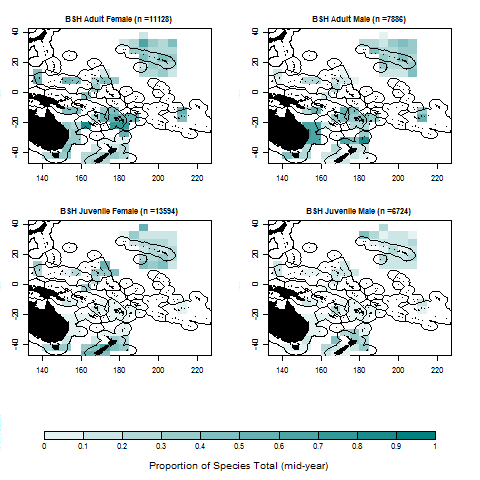
\includegraphics[width=\textwidth]{../GRAPHICS/Defined/BI_20_Map_maturity_sex_BSH_MY}
       \caption{Mid-year estimates.}
       \label{fig:test1}
   \end{subfigure}
   \begin{subfigure}[b]{0.6\textwidth}
       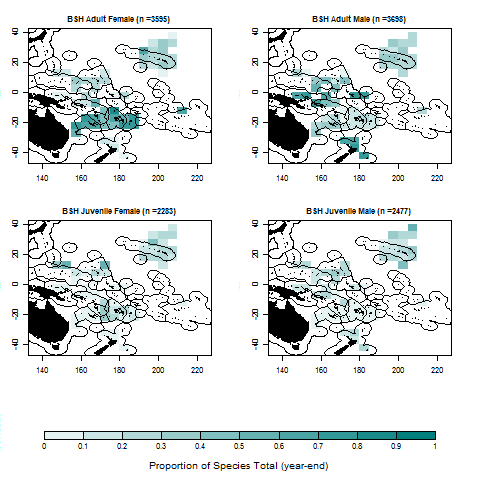
\includegraphics[width=\textwidth]{../GRAPHICS/Defined/BI_19_Map_maturity_sex_BSH}
       \caption{End of year estimates.}
       \label{fig:test2}
   \end{subfigure}
\caption{Blue Shark:  Proportion observed in each 5 x 5 degree cell which were adult females, adult males, juvenile females and juvenile males for mid-year (left panel) and year-end (right panel) periods. Darker cell shading indicates higher proportions observed. Samples sizes shown are those before removing cells with less than 20 individuals from the analysis. }
\label{BI_01} 
\end{figure}
\end{landscape}


%% Silky
\begin{landscape}
\begin{figure}
\centering
   \begin{subfigure}[b]{0.6\textwidth}
       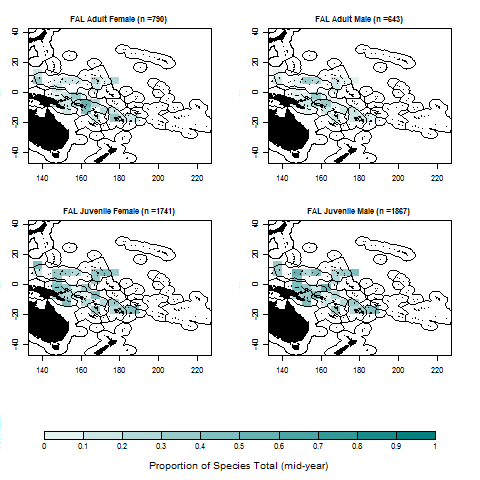
\includegraphics[width=\textwidth]{../GRAPHICS/Defined/BI_22_Map_maturity_sex_FAL_MY}
       \caption{Mid-year estimates.}
       \label{fig:test1}
   \end{subfigure}
   \begin{subfigure}[b]{0.6\textwidth}
       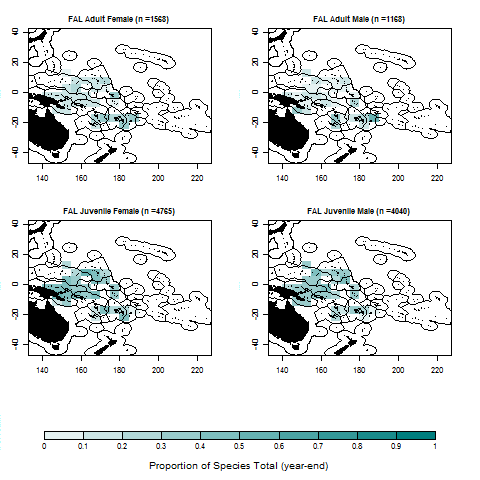
\includegraphics[width=\textwidth]{../GRAPHICS/Defined/BI_21_Map_maturity_sex_FAL}
       \caption{End of year estimates.}
       \label{fig:test2}
   \end{subfigure}
\caption{Silky Shark: Proportion observed in each 5 x 5 degree cell which were adult females, adult males, juvenile females and juvenile males for mid-year (left panel) and year-end (right panel) periods. Darker cell shading indicates higher proportions observed. Samples sizes shown are those before removing cells with less than 20 individuals from the analysis. }
\label{fig:test} 
\end{figure}
\end{landscape}

%% Hammerhead
\begin{landscape}
\begin{figure}
\centering
   \begin{subfigure}[b]{0.6\textwidth}
       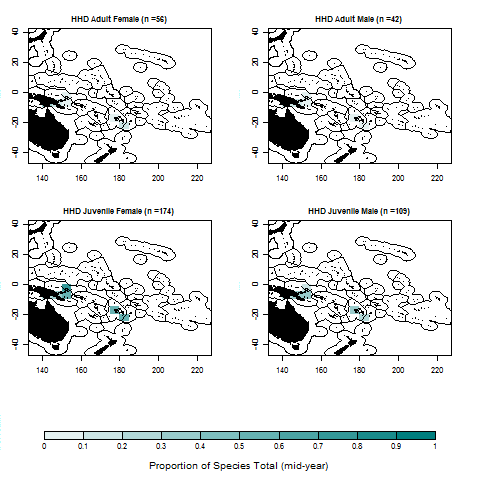
\includegraphics[width=\textwidth]{../GRAPHICS/Defined/BI_24_Map_maturity_sex_HHD_MY}
       \caption{Mid-year estimates.}
       \label{fig:test1}
   \end{subfigure}
   \begin{subfigure}[b]{0.6\textwidth}
       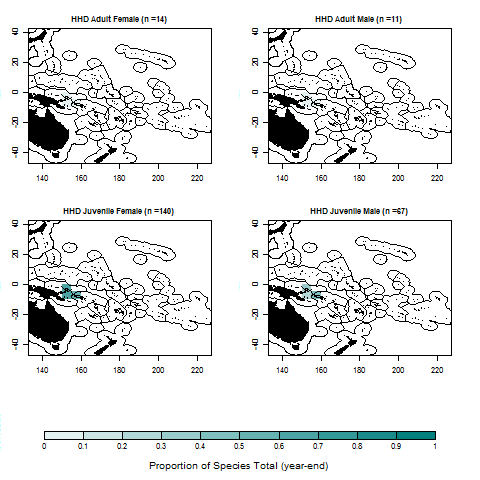
\includegraphics[width=\textwidth]{../GRAPHICS/Defined/BI_23_Map_maturity_sex_HHD}
       \caption{End of year estimates.}
       \label{fig:test2}
   \end{subfigure}
\caption{Hammerhead Shark: Proportion observed in each 5 x 5 degree cell which were adult females, adult males, juvenile females and juvenile males for mid-year (left panel) and year-end (right panel) periods. Darker cell shading indicates higher proportions observed. Samples sizes shown are those before removing cells with less than 20 individuals from the analysis. }
\label{fig:test} 
\end{figure}
\end{landscape}

%% Mako
\begin{landscape}
\begin{figure}
\centering
   \begin{subfigure}[b]{0.6\textwidth}
       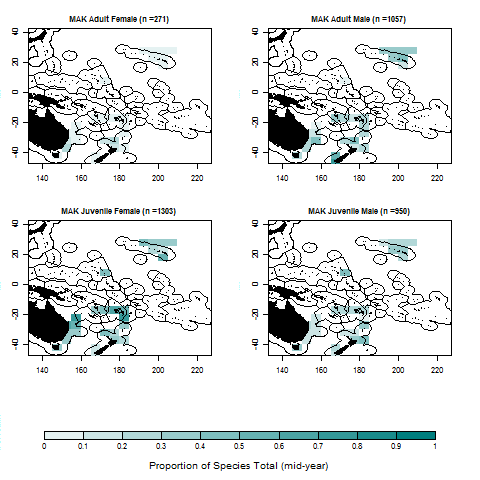
\includegraphics[width=\textwidth]{../GRAPHICS/Defined/BI_26_Map_maturity_sex_MAK_MY}
       \caption{Mid-year estimates.}
       \label{fig:test1}
   \end{subfigure}
   \begin{subfigure}[b]{0.6\textwidth}
       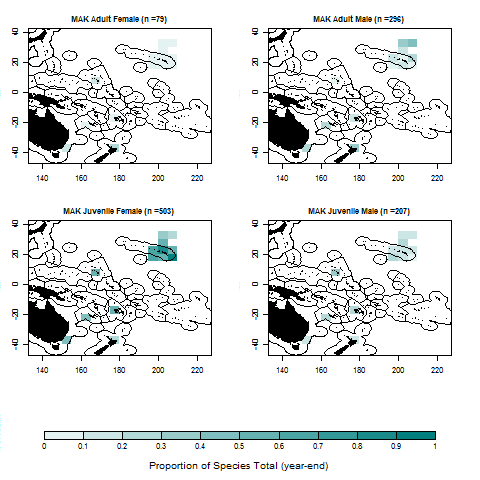
\includegraphics[width=\textwidth]{../GRAPHICS/Defined/BI_25_Map_maturity_sex_MAK}
       \caption{End of year estimates.}
       \label{fig:test2}
   \end{subfigure}
\caption{Mako Shark: Proportion observed in each 5 x 5 degree cell which were adult females, adult males, juvenile females and juvenile males for mid-year (left panel) and year-end (right panel) periods. Darker cell shading indicates higher proportions observed. Samples sizes shown are those before removing cells with less than 20 individuals from the analysis. }
\label{fig:test} 
\end{figure}
\end{landscape}

%% OCS
\begin{landscape}
\begin{figure}
\centering
   \begin{subfigure}[b]{0.6\textwidth}
       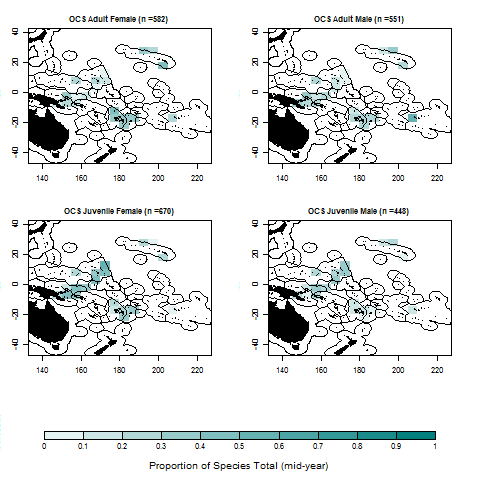
\includegraphics[width=\textwidth]{../GRAPHICS/Defined/BI_28_Map_maturity_sex_OCS_MY}
       \caption{Mid-year estimates.}
       \label{fig:test1}
   \end{subfigure}
   \begin{subfigure}[b]{0.6\textwidth}
       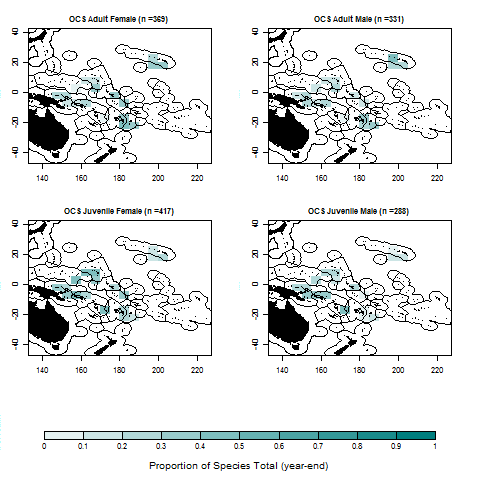
\includegraphics[width=\textwidth]{../GRAPHICS/Defined/BI_27_Map_maturity_sex_OCS}
       \caption{End of year estimates.}
       \label{fig:test2}
   \end{subfigure}
\caption{Oceanic Whitetip Shark: Proportion observed in each 5 x 5 degree cell which were adult females, adult males, juvenile females and juvenile males for mid-year (left panel) and year-end (right panel) periods. Darker cell shading indicates higher proportions observed. Samples sizes shown are those before removing cells with less than 20 individuals from the analysis. }
\label{fig:test} 
\end{figure}
\end{landscape}

%% Porbeagle
\begin{landscape}
\begin{figure}
\centering
   \begin{subfigure}[b]{0.6\textwidth}
       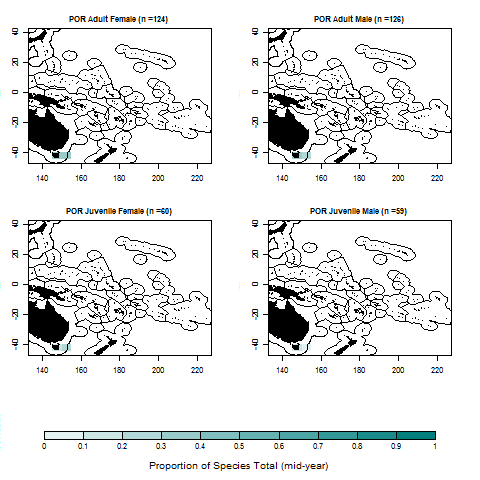
\includegraphics[width=\textwidth]{../GRAPHICS/Defined/BI_30_Map_maturity_sex_POR_MY}
       \caption{Mid-year estimates.}
       \label{fig:test1}
   \end{subfigure}
   \begin{subfigure}[b]{0.6\textwidth}
       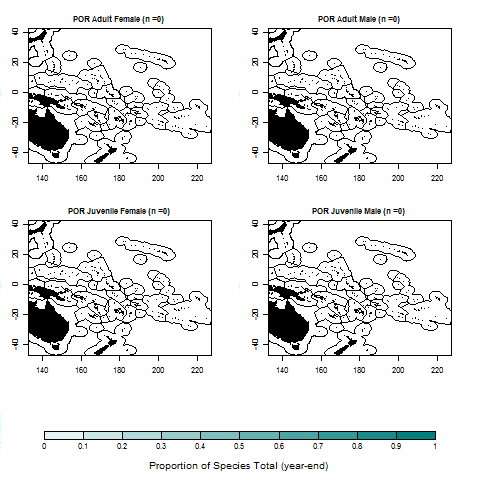
\includegraphics[width=\textwidth]{../GRAPHICS/Defined/BI_29_Map_maturity_sex_POR}
       \caption{End of year estimates.}
       \label{fig:test2}
   \end{subfigure}
\caption{Porbeagle Shark: Proportion observed in each 5 x 5 degree cell which were adult females, adult males, juvenile females and juvenile males for mid-year (left panel) and year-end (right panel) periods. Darker cell shading indicates higher proportions observed. Samples sizes shown are those before removing cells with less than 20 individuals from the analysis. }
\label{fig:test} 
\end{figure}
\end{landscape}

%% Thresher
\begin{landscape}
\begin{figure}
\centering
   \begin{subfigure}[b]{0.6\textwidth}
       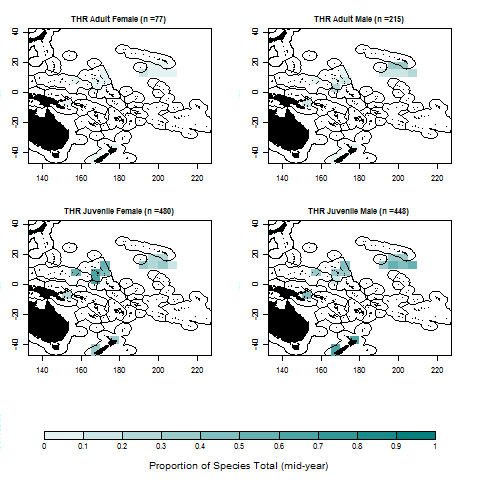
\includegraphics[width=\textwidth]{../GRAPHICS/Defined/BI_32_Map_maturity_sex_THR_MY}
       \caption{Mid-year estimates.}
       \label{fig:test1}
   \end{subfigure}
   \begin{subfigure}[b]{0.6\textwidth}
       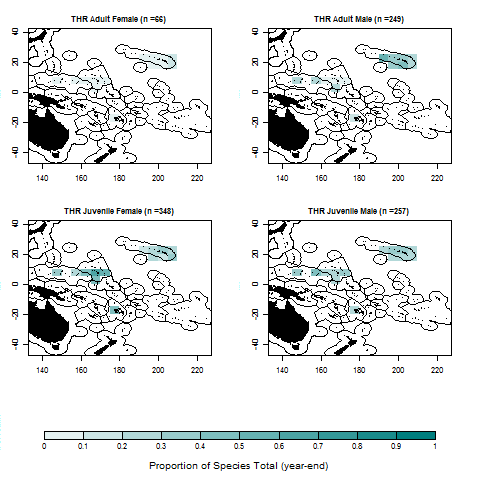
\includegraphics[width=\textwidth]{../GRAPHICS/Defined/BI_31_Map_maturity_sex_THR}
       \caption{End of year estimates.}
       \label{fig:test2}
   \end{subfigure}
\caption{Thresher Shark: Proportion observed in each 5 x 5 degree cell which were adult females, adult males, juvenile females and juvenile males for mid-year (left panel) and year-end (right panel) periods. Darker cell shading indicates higher proportions observed. Samples sizes shown are those before removing cells with less than 20 individuals from the analysis. }
\label{fig:test} 
\end{figure}
\end{landscape}

%%%%%%%%%%%%%%%%%%%%%%%%%%%%%%%%%%%%%%%%%%%%%%%%%%%%%%%%%%%%%%%%%%%%%%%%%%%%%%%%%%%%%%%%%%%%%%%%%%%%%%%%%%%%%%%%%%%%%%%%%%
\clearpage
\section{Whale Shark Figures}
\addcenterfig[Annual number of observed free school sets (bars) and proportion of sets with some form of whale shark interaction (see text for criteria).]{fig:whaleshark1}{../GRAPHICS/Whale-Shark-Picture-1}

\addcenterfig[Contour plots based on 1 $\times$ 1 degree square data for all years combined of purse seine sets (top), whale shark records (middle – see text for criteria), and encounter rates (bottom --- simply whale shark records divided by total sets for each 1 x1 degree square). Grey represents zeros, white are NA’s (e.g. zero whale sharks divided by zero sets), and the scale increases from green to yellow to orange to pink to red.]{fig:whaleshark2}{../GRAPHICS/Whale-Shark-Picture-2}
%%%%%%%%%%%%%%%%%%%%%%%%%%%%%%%%%%%%%%%%%%%%%%%%%%%%%%%%%%%%%%%%%%%%%%%%%%%%%%%%%%%%%%%%%%%%%%%%%%%%%%%%%%%%%%%%%%%%%%%%%%
\clearpage
\section{Management Considerations}

\addcenterfig[Fate of observed sharks caught by longline in the WCPO (total numbers for all species combined).]{fig:map}{../GRAPHICS/fate_ll_obs_by_region}

\addcenterfig[Fate of observed sharks caught by longline in the WCPO (proportion by number for all species combined).]{fig:map}{../GRAPHICS/fate_ll_ps_obs_all_keysharks_wcpo}


\addcenterfig[Fate of observed blue sharks caught by longline in the WCPO.]{fig:map}{../GRAPHICS/fate_ll_obs_BSH}
\addcenterfig[Fate of observed silky sharks caught by longline in the WCPO.]{fig:map}{../GRAPHICS/fate_ll_obs_FAL}
\addcenterfig[Fate of observed hammerhead sharks caught by longline in the WCPO.]{fig:map}{../GRAPHICS/fate_ll_obs_HHD}
\addcenterfig[Fate of observed mako sharks caught by longline in the WCPO.]{fig:map}{../GRAPHICS/fate_ll_obs_MAK}
\addcenterfig[Fate of observed oceanic whitetip sharks caught by longline in the WCPO.]{fig:map}{../GRAPHICS/fate_ll_obs_OCS}
\addcenterfig[Fate of observed porbeagle sharks caught by longline in the WCPO.]{fig:map}{../GRAPHICS/fate_ll_obs_POR}
\addcenterfig[Fate of observed thresher sharks caught by longline in the WCPO.]{fig:map}{../GRAPHICS/fate_ll_obs_THR}


\section{Model Diagnostics}
\subsubsection{CPUE Standardisation Diagnostics}

\addcenterfig[CPUE indicators, model diagnostics for blue shark (north) CPUE standardization via negative binomial model.]{fig:diagno1}{../GRAPHICS/BSH.north_MU~yy+program_code + HPBCAT2 + mm + sharkbait_SIGMA~program_code + HPBCAT2 + mm_resids}

\addcenterfig[CPUE indicators, model diagnostics for blue shark (north) CPUE standardization via negative binomial model.]{fig:map}{../GRAPHICS/SHK-GLM-vars-bp-smry_BSH.north}


\addcenterfig[CPUE indicators, model diagnostics for blue shark (south) CPUE standardization via negative binomial model.]{fig:map}{../GRAPHICS/BSH.south_MU~yy+flag + HPBCAT2 + mm + sharkbait_SIGMA~intrcpt_resids}

\addcenterfig[CPUE indicators, model diagnostics for blue shark (south) CPUE standardization via negative binomial model.]{fig:map}{../GRAPHICS/SHK-GLM-vars-bp-smry_BSH.south}


\addcenterfig[CPUE indicators, model diagnostics for silky shark CPUE standardization via negative binomial model.]{fig:map}{../GRAPHICS/FAL_MU~yy+program_code + HPBCAT2 + mm + sharkbait_SIGMA~program_code + sharkbait + mm_resids}

\addcenterfig[CPUE indicators, model diagnostics for silky shark CPUE standardization via negative binomial model.]{fig:map}{../GRAPHICS/SHK-GLM-vars-bp-smry_FAL}

\clearpage
\addcenterfig[CPUE indicators, model diagnostics for hammerhead shark CPUE standardization via negative binomial model]{fig:map}{../GRAPHICS/HHD_MU~yy+program_code + HPBCAT2 + mm + sharkbait_SIGMA~sharkbait_resids}

\addcenterfig[CPUE indicators, model diagnostics for hammerhead shark CPUE standardization via negative binomial model]{fig:map}{../GRAPHICS/SHK-GLM-vars-bp-smry_HHD}


\addcenterfig[CPUE indicators, model diagnostics for mako shark (northern hemisphere) CPUE standardization via negative binomial model.]{fig:map}{../GRAPHICS/MAK.north_MU~yy+program_code + mm + sharkbait_SIGMA~HPBCAT2_resids}

\addcenterfig[CPUE indicators, model diagnostics for mako shark (northern hemisphere) CPUE standardization via negative binomial model.]{fig:makoStdCPUEvars}{../GRAPHICS/SHK-GLM-vars-bp-smry_MAK.north}


\addcenterfig[CPUE indicators, model diagnostics for mako shark (southern hemisphere) CPUE standardization via negative binomial model.]{fig:makoStdCPUEvars2}{../GRAPHICS/MAK.south_MU~yy+program_code + HPBCAT2 + mm + sharkbait_SIGMA~program_code + mm_resids}

\addcenterfig[CPUE indicators, model diagnostics for mako shark (southern hemisphere) CPUE standardization via negative binomial model.]{fig:map}{../GRAPHICS/SHK-GLM-vars-bp-smry_MAK.south}


\addcenterfig[CPUE indicators, model diagnostics for oceanic whitetip shark CPUE standardization via negative binomial model.]{fig:map}{../GRAPHICS/OCS_MU~yy+program_code + HPBCAT2 + mm + sharkbait_SIGMA~program_code_resids}

\addcenterfig[CPUE indicators, model diagnostics for oceanic whitetip shark CPUE standardization via negative binomial model.]{fig:map}{../GRAPHICS/SHK-GLM-vars-bp-smry_OCS}

\addcenterfig[CPUE indicators, model diagnostics for porbeagle shark CPUE standardization via negative binomial model.]{fig:map}{../GRAPHICS/POR_MU~yy + flag + HPBCAT2 + mm_SIGMA~flag + mm_resids}

\addcenterfig[CPUE indicators, model diagnostics for porbeagle shark CPUE standardization via negative binomial model.]{fig:map}{../GRAPHICS/SHK-GLM-vars-bp-smry_POR}


\addcenterfig[CPUE indicators, model diagnostics for thresher CPUE standardization via negative binomial model.]{fig:map}{../GRAPHICS/THR_MU~yy+program_code + HPBCAT2 + mm_SIGMA~HPBCAT2 + program_code_resids}

\addcenterfig[CPUE indicators, model diagnostics for thresher CPUE standardization via negative binomial model.]{fig:diagno2}{../GRAPHICS/SHK-GLM-vars-bp-smry_THR}

\clearpage
\BSHnorthaic
\BSHsouthaic
\FALaic
\HHDaic
\MAKnorthaic
\MAKsouthaic
\OCSaic
\PORaic
\THRaic

%%%%%%%%%%%%%%%%%%%%%%%%%%%%%%%%%%%%%%%%%%
% SC Information Paper 5 
% SHARK INDICATORS IN THE WESTERN CENTRAL PACIFIC
% June 2015
%
% Author: Joel Rice (joelrice@uw.edu )
%
%
%%%%%%%%%%%%%%%%%%%%%%%%%%%%%%%%%%%%%%%%%

%----------------------------------------------------------------------------------------
%  PACKAGES AND OTHER DOCUMENT CONFIGURATIONS
%----------------------------------------------------------------------------------------



%\documentclass[12pt]{SCreport}

%\usepackage{fullpage}
\usepackage{amssymb, amsmath}
\usepackage{natbib}
\usepackage{booktabs}
\usepackage{url}
\usepackage{setspace}
\usepackage{hyperref}
%\usepackage{gensymb}
\usepackage{pdflscape}
\usepackage{etoolbox}
\usepackage[utf8]{inputenc}
\usepackage{graphicx}
\usepackage{caption}
\usepackage{parskip}
\usepackage[margin=1in]{geometry} % customize margins 
\usepackage{parskip} % one line between paragraphs
\usepackage{grffile} % allows ~, . ,etc. into figure file names

\usepackage{comment}
\usepackage[usenames,dvipsnames,svgnames]{xcolor}
\usepackage{soul}
\usepackage{xspace}


\onehalfspacing



% normal figure, centred in page
\newcommand{\capnow}{}
\newcommand{\addcenterfig}[3][Caption to be completed]{
  \begin{figure}[!h]
    \begin{center}
      \includegraphics[width=\textwidth]{#3}
     \caption{#1 \label{#2}}
    \end{center}
  \end{figure}
}

% landscape figure
\newcommand{\addcenterfigLS}[3][Caption to be completed]{
 \newgeometry{left=0.5cm,bottom=2.5cm,right=1cm,top=2.5cm}

\begin{landscape}
%\topskip0pt
   \vspace*{\fill}

\begin{figure}[!h]
    \begin{center}
      \includegraphics[width=620pt]{#3}
     \caption{#1 \label{#2}}
    \end{center}

  \end{figure}
  \vspace*{\fill}

\clearpage
\end{landscape}
\restoregeometry
}

%\graphicspath{ {C:/Projects/SHK-indicators-2015/GRAPHICS/}{C:/Projects/SHK-indicators-2015/GRAPHICS/CPUE_std/} }

%\usepackage[english]{babel}

%%%%%%%%%%%%%%%%%%%%%%%%%%%%%%%%%%%%%%%%%%%%%%%%%%%%%%%%%%%%%
%%%%%%%%%%%%%%%%%%%%% WCPFC title page %%%%%%%%%%%%%%%%%%%%% 
%% Commands for users to define title page settings
\newcommand{\spcauthor}{Use \textbackslash reportauthor to defined report authors}
\newcommand{\reportauthor}[1]{\renewcommand{\spcauthor}{#1}}

\newcommand{\spctitle}{Use \textbackslash reporttitle to defined report authors}
\newcommand{\reporttitle}[1]{\renewcommand{\spctitle}{#1}}

\newcommand{\repnumbr}{Use \textbackslash reportnumber to defined report authors}
\newcommand{\reportnumber}[1]{\renewcommand{\repnumbr}{#1}}

%% define title page macro 
\newcommand{\wcpfctitlepage}{

\thispagestyle{empty}
\begin{center}
\begin{figure}
\begin{center}

\includegraphics[scale=0.6]{WCPFC-logo.jpg}

\end{center}
\end{figure}
\textbf{SCIENTIFIC COMMITTEE\\ELEVENTH REGULAR SESSION\\}
Pohnpei, Federated States of Micronesia\\
5--13 August 2015\\

\vspace{0.5in}
\rule{\textwidth}{0.5mm}
%\vspace{-0.25cm}
\bfseries{\spctitle} % report title inserted here
\rule{\textwidth}{0.5mm}
\end{center}

\begin{flushright}
\textbf{WCPFC-SC11-2015/\repnumbr} % report number
\end{flushright}
\vspace{1in}

\begin{center} % report authors
\textbf{\spcauthor \footnote{\label{spc-ref}Oceanic Fisheries Programme, Secretariat of the Pacific Community}}
\end{center}

\clearpage}
%\reportauthor{Joel Rice\footnote{Joel Rice Consulting Ltd.}, Laura Tremblay-Boyer, and Shelton Harley}
%\reporttitle{Analysis of stock status and related indicators for key shark species of the Western Central Pacific Fisheries Commission}
%\reportnumber{SA-IP-05}



%----------------------------------------------------------------------------------------
%  Document content
%----------------------------------------------------------------------------------------

%\begin{document}

%----------------------------------------------------------------------------------------

\subsection{Longline Fishery Data}
%---------------------------------------------------------------------------------------------

\addcenterfig[Map of WCPO and observed effort. ]{fig:LLsets}{FIG_2_MAP_sets}

 
\addcenterfig[Total number of hooks fished by flag (for the top four fishing nations, and all others combined) based on   aggregated (5x5 degree square) data, for six regions of the WCPFC Statistical Area. ]{fig:LLLogbood_flag_hooks}{FIG_xx_LLeff_FLAG}
 

\addcenterfig[Total number of reported sharks  by flag (for the top four fishing nations, and all others combined) based aggregated (5x5 degree square) data, for six regions of the WCPFC Statistical Area.]{fig:LLLog_flag_shks}{FIG_xx_LLreported_catch_FLAG}
 

\addcenterfig[Total number of hooks observed by flag (for the top four fishing nations) based on longline observer records held by the SPC-OFP, for six regions of the WCPFC Statistical Area  ]{fig:obsLL_flag}{FIG_xx_LLeff_FLAG}    

\addcenterfig[Logsheet effort by month.]{fig:logeffmnth}{FIG_xx_LOGSHEET_mm}
\addcenterfig[Observed effort by month.]{fig:obseffmnth}{FIG_xx_obsBY_mm}
\addcenterfig[Absolute percent difference in effort between reported (logsheet)  effort and observed effort.]{fig:effdiff}{FIG_xx_obsDIFFlog_mm}


\clearpage

              
\addcenterfig[Aggregate effort by region. ]{fig:aggeff}{FIG_xx_agg_eff}
%\addcenterfig[Observed effort by region.]{fig:obseff}{FIG_xx_OBS_eff}

\addcenterfig[Observed purse seine in the  WCPO showing the top four fishing nations and all others combined.  ]{fig:pssets}{FIG_xx_PS_eMAP_sets}

%-------------------------------------------------------------------------------------------------------------------------
 
 \subsubsection*{Fishing Effort- Purse Seine} 
 
 \addcenterfig[Absolute percent difference in effort between reported (logsheet)  effort and observed effort.]{fig:seine_map}{FIG_xx_PS_sets}
 
 
 \addcenterfig[Comparison by region and flag of purse seine effort (in sets) associated sets using aggregated (5x5 degree square) data for six regions of the WCPFC Statistical Area, excluding data from Indonesia, Vietnam, and Japan coastal waters.]{fig:ps_ass_eff}{ps_total_effAssociated}
  \addcenterfig[Comparison by region and flag of purse seine effort (in sets) unassociated sets using aggregated (5x5 degree square) data for six regions of the WCPFC Statistical Area, excluding data from Indonesia, Vietnam, and Japan coastal waters.]{fig:ps_una_eff}{ps_total_effUnassociated} 

 \addcenterfig[Total sharks recorded on logsheets (in number of sets recording at least one shark interaction), for associated sets.]{fig:log_ass_shk}{ps_oper_shks_rep_cntry_associated}
 \addcenterfig[Total sharks recorded on logsheets (in number of sets recording at least one shark interaction), for unassociated sets.]{fig:log_una_shk}{ps_oper_shks_rep_cntry_unassociated} 
 
 
 
 
\clearpage         
 %       \subsection{Data formatting}
 %       \subsection{Limitations - Caveats}
        
        
%----------------------------------------------------------------------------------------
%  Distribuion Indicators
%----------------------------------------------------------------------------------------
             
        
\section{Distribution Indicator Analyses}
      \subsection{Introduction}
      \subsection{Methods}
      \subsection{Results}
         

\clearpage         
%----------------------------------------------------------------------------------------
          \subsubsection{Blue Shark}

\addcenterfig[Blue shark distribution indicators. Proportion of positive sets, observer data.]{fig:bsh1}{FIG_xx_pcntpos_reg_BSH}
\addcenterfig[Blue shark distribution indicators. Proportion of 5 degree squares having CPUE greater than 1 per 1000 hooks region, observer data.]{fig:bsh2}{FIG_xx_HIGH_CPUE_BSH}


%----------------------------------------------------------------------------------------
\subsubsection{Mako Shark}

\addcenterfig[Mako shark distribution indicators. Proportion of positive sets, observer data.]{fig:mak1}{FIG_xx_pcntpos_reg_MAK}          
\addcenterfig[Mako shark distribution indicators. Proportion of 5 degree squares having CPUE greater than 1 per 1000 hooks region, observer data.]{fig:mak2}{FIG_xx_HIGH_CPUE_MAK}
          
          
%----------------------------------------------------------------------------------------
 \subsubsection{Silky Shark}
 
\addcenterfig[Mako shark distribution indicators. Proportion of positive sets, observer data.]{fig:fal1}{FIG_xx_pcntpos_reg_FAL}           
\addcenterfig[Silky shark distribution indicators. Proportion of 5 degree squares having CPUE greater than 1 per 1000 hooks region, observer data.]{fig:fal2}{FIG_xx_HIGH_CPUE_FAL}

%----------------------------------------------------------------------------------------
 \subsubsection{Oceanic Whitetip Shark}
 \addcenterfig[Oceanic whitetip shark distribution indicators. Proportion of positive sets, observer data.]{fig:ocs1}{FIG_xx_pcntpos_reg_OCS}          
 \addcenterfig[Oceanic whitetip shark distribution indicators. Proportion of 5 degree squares having CPUE greater than 1 per 1000 hooks region, observer data.]{fig:ocs2}{FIG_xx_HIGH_CPUE_OCS}

%----------------------------------------------------------------------------------------
 \subsubsection{Thresher Shark}
\addcenterfig[Thresher shark distribution indicators. Proportion of positive sets, observer data.]{fig:thr1}{FIG_xx_pcntpos_reg_THR} 
\addcenterfig[Thresher shark distribution indicators. Proportion of 5 degree squares having CPUE greater than 1 per 1000 hooks region, observer data.]{fig:thr2}{FIG_xx_HIGH_CPUE_THR}
          
%----------------------------------------------------------------------------------------
 \subsubsection{Hammerhead Shark}
\addcenterfig[Hammerhead shark distribution indicators. Proportion of positive sets, observer data.]{fig:HHD1}{FIG_xx_pcntpos_reg_HHD} 
\addcenterfig[Hammerhead shark distribution indicators. Proportion of 5 degree squares having CPUE greater than 1 per 1000 hooks region, observer data.]{fig:HHD2}{FIG_xx_HIGH_CPUE_HHD}

%----------------------------------------------------------------------------------------
\subsubsection{Porbeagle Shark}
\addcenterfig[Porbeagle shark distribution indicators. Proportion of positive sets, observer data.]{fig:POR1}{FIG_xx_pcntpos_reg_POR} 
\addcenterfig[Porbeagle shark distribution indicators. Proportion of 5 degree squares having CPUE greater than 1 per 1000 hooks region, observer data.]{fig:POR2}{FIG_xx_HIGH_CPUE_POR}

  \subsection{Conclusions}
%----------------------------------------------------------------------------------------
%  Species COmposition
%----------------------------------------------------------------------------------------
      
      
\section{Observed Species Composition Indicator Analyses}
      \subsection{Introduction}
      \subsection{Methods}
      \subsection{Results}
      
  \subsubsection*{Longline}      
  \addcenterfig[Catch Composition Indicators. Sharks Per. 1000 hooks by region, observer data.]{fig:catchcomp1}{FIG_xx_shksP1000Hooks}
  \addcenterfig[Catch Composition Indicators. Sharks Per. 1000 hooks by region, deep sets observer data.]{fig:catchcomp2}{FIG_xx_shksP1000Hooks_deep}  
  \addcenterfig[Catch Composition Indicators. Sharks Per. 1000 hooks by region, shallow sets observer data.]{fig:catchcomp3}{FIG_xx_shksP1000Hooks_shallow}
  \addcenterfig[Catch Composition Indicators. Proportional catch of main species and other sharks by retions.]{fig:catchcomp3a}{catchcomp_xx_llshks_pcnt}
  
  
%------------------------------------------------------------------------------------------
\clearpage
 \subsubsection*{Purse Seine}        
 \addcenterfig[Catch Composition Indicators. Sharks per set, observer data.]{fig:catchcomp4}{FIG_xx_PS_shks_set}
 \addcenterfig[Catch Composition Indicators. Sharks per set, associated sets, observer data]{fig:catchcomp5}{FIG_xx_PS_shks_UNAS}  
 \addcenterfig[Catch Composition Indicators. Sharks per set, unassociated sets, observer data.]{fig:catchcomp6}{FIG_xx_PS_shks_ASSO} 

  \addcenterfig[Catch Composition Indicators. Catch composition by proportion , observer data.]{fig:catchcomp7}{catchcomp_xx_PS_comp_reg}
 \addcenterfig[Catch Composition Indicators. Catch composition by proportion, associated sets, observer data]{fig:catchcomp8}{catchcomp_xx_PS_comp_reg_UNAS}  
 \addcenterfig[Catch Composition Indicators. Catch composition by proportion, unassociated sets, observer data.]{fig:catchcomp9}{catchcomp_xx_PS_comp_reg_ASSOC} 

 
 
 \subsection{Conclusions}
      
      
 \clearpage          

%----------------------------------------------------------------------------------------
%  CPUE INDICATORS
%----------------------------------------------------------------------------------------
\section{Catch Per Unit Effort indicator analyses}

\subsection*{Purse Seine data preparation}

\addcenterfig[CPUE indicators, nominal CPUE in the purse seine fishery, all sets, Region 3.]{fig:cpue_ps1}{cpue_psnom_reg3}
\addcenterfig[CPUE indicators, nominal CPUE in the purse seine fishery, all sets, Region 4.]{fig:cpue_ps2}{cpue_psnom_reg4}






%----------------------------------------------------------------------------------------
%----------------------------------------------------------------------------------------
\clearpage  
\subsection{Results}
    %----------------------------------------------------------------------------------------

  \subsubsection{Blue Shark}
           
\addcenterfig[Blue shark CPUE indicators. Proportion of positive sets, observer data.]{fig:bshcp1}{FIG_xx_pcntpos_reg_BSH}
\addcenterfig[Blue shark CPUE indicators. Nominal CPUE, sharks per 1000 hooks, observer data.]{fig:bshcp2}{FIG_xx_nomCPUE_reg_BSH}


% \addcenterfig[Blue shark CPUE indicators. Standardized blue shark CPUE based on the negative binomial model for observer data in the northern hemisphere.]{fig:bshcp3}{LLcpue_BSH_north_NB_step}
% 
% \addcenterfig[Blue shark CPUE indicators. Standardized CPUE, zero inflated negative binomial Southern Hemisphere, observer data.]{fig:bshcp4}{ll_cpue_BSHzinb_nominal}
% 
%  



%----------------------------------------------------------------------------------------
 \subsubsection{Mako Shark}
%           
 \addcenterfig[Mako shark CPUE indicators. Proportion of positive sets, observer data.]{fig:makcp1}{FIG_xx_pcntpos_reg_MAK}
  \addcenterfig[Mako shark CPUE indicators. Nominal CPUE, sharks per 1000 hooks, observer data.]{fig:makcp2}{FIG_xx_nomCPUE_reg_MAK}
% 
% \addcenterfig[Mako shark CPUE indicators. Standardized CPUE, mako shark in the northern hemisphere.]{fig:makcp3}{LLcpue_MAKO_north_NB_cpue}
% \addcenterfig[Mako shark CPUE indicators. Standardized CPUE, mako shark in the southern hemisphere.]{fig:makcp4}{LLcpue_MAKO_southth_NB_cpue}


\clearpage
%----------------------------------------------------------------------------------------
\subsubsection{Silky Shark}

  \addcenterfig[Silky shark CPUE indicators. Proportion of positive sets, observer data.]{fig:falcp1}{FIG_xx_pcntpos_reg_FAL}
 \addcenterfig[Silky shark CPUE indicators. Nominal CPUE, sharks per 1000 hooks, observer data.]{fig:falcp2}{FIG_xx_nomCPUE_reg_FAL}
% \addcenterfig[Silky shark CPUE indicators. Standardized CPUE from longline observer data for silky sharks.]{fig:falcp3}{LLcpue_FAL_NB_cpue}



%----------------------------------------------------------------------------------------
\subsubsection{Oceanic Whitetip Shark}
%           
 \addcenterfig[Oceanic whitetip shark CPUE indicators. Proportion of positive sets, observer data.]{fig:ocscp1}{FIG_xx_pcntpos_reg_OCS}
 \addcenterfig[Oceanic whitetip shark CPUE indicators. Nominal CPUE, sharks per 1000 hooks, observer data.]{fig:ocscp2}{FIG_xx_nomCPUE_reg_OCS}
% \addcenterfig[Oceanic whitetip shark CPUE indicators. Standardized CPUE based on negative  binomial models applied to observer data.]{fig:ocscp3}LLcpue_OCS_NB_cpue}


%----------------------------------------------------------------------------------------
  \subsubsection{Thresher Shark}
          
 \addcenterfig[Thresher shark CPUE indicators. Proportion of positive sets, observer data.]{fig:thrcp1}{FIG_xx_pcntpos_reg_THR}
 \addcenterfig[Thresher shark CPUE indicators. Nominal CPUE, sharks per 1000 hooks, observer data.]{fig:thrcp2}{FIG_xx_nomCPUE_reg_THR}
% \addcenterfig[Thresher shark CPUE indicators.  Standardized CPUE of thresher shark based on longline observer data.]{fig:thrcp3}{LLcpue_THRESHER_NB_cpue}


%----------------------------------------------------------------------------------------          
%----------------------------------------------------------------------------------------
  \subsubsection{Hammerhead Shark}
          
 \addcenterfig[Thresher shark CPUE indicators. Proportion of positive sets, observer data.]{fig:HHDcp1}{ }
 \addcenterfig[Thresher shark CPUE indicators. Nominal CPUE, sharks per 1000 hooks, observer data.]{fig:HHDcp2}{ }
% \addcenterfig[Thresher shark CPUE indicators.  Standardized CPUE of thresher shark based on longline observer data.]{fig:thrcp3}{LLcpue_THRESHER_NB_cpue}
   
     \subsubsection{Hammerhead Shark}
          
 \addcenterfig[Thresher shark CPUE indicators. Proportion of positive sets, observer data.]{fig:HHDcp1}{ }
 \addcenterfig[Thresher shark CPUE indicators. Nominal CPUE, sharks per 1000 hooks, observer data.]{fig:HHDcp2}{ }
% \addcenterfig[Thresher shark CPUE indicators.  Standardized CPUE of thresher shark based on longline observer data.]{fig:thrcp3}{LLcpue_THRESHER_NB_cpue}
      
   
 \clearpage     
      
      
      
      
     
%----------------------------------------------------------------------------------------
%  Biological
%----------------------------------------------------------------------------------------
      
\section{Biological indicator analyses}
     
      
%----------------------------------------------------------------------------------------
%  Discussion Type Sections.........
%----------------------------------------------------------------------------------------
         
      
\section{Feasibility of Stock Assessments}
\section{Impact of Recent Shark Management Measures}
 % analysis of fate and condition goes here? 

\section{Recommendations for Future Indicator Work}
\section{Management Implications}

\section*{Acknowledgements}
\clearpage
%----------------------------------------------------------------------------------------
%  REFERENCE LIST
%----------------------------------------------------------------------------------------


%----------------------------------------------------------------------------------------
%  Appendices 
%----------------------------------------------------------------------------------------

\section{Appendices}
% 
\subsection{CPUE Indicators.  Model diagnostics and extra plots}

% \addcenterfig[CPUE indicators, nominal CPUE in the purse seine fishery, Unassociated Sets, Region 3.]{fig:cpue_ps_an1}{cpue_psnom_reg3_UNASS}
% \addcenterfig[CPUE indicators, nominal CPUE in the purse seine fishery, Unassociated sets, Region 4.]{fig:cpue_ps_an2}{cpue_psnom_reg4_UNASS}
% 
% \addcenterfig[CPUE indicators, nominal CPUE in the purse seine fishery, Associated Sets, Region 3.]{fig:cpue_ps_an3}{cpue_psnom_reg3_assoc}
% \addcenterfig[CPUE indicators, nominal CPUE in the purse seine fishery, Associated sets, Region 4.]{fig:cpue_ps_an4}{cpue_psnom_reg4_assoc}

%----------------------------------------------------------------------------------------
 \subsubsection*{Blue Shark model diagnostics and extra plots}

%%%   Missing \addcenterfig[CPUE indicators, GLM model diagnostics BSH in the North Pacific.]{fig:cpue_bsh_an1}{BSH_NB_N_diag}
%   
%   \addcenterfig[CPUE indicators, GLM model diagnostics .]{fig:cpue_BSH_an2}{BSH_ZINB_S_diag}
%   
%   \addcenterfig[CPUE indicators, GLM model diagnostics, BSH in the north Pacific step plot.]{fig:cpue_BSH_an3}{LLcpue_BSH_north_NB_step}
%   \addcenterfig[CPUE indicators, GLM model diagnostics, BSH in the south Pacific step plot.]{fig:cpue_BSH_an4}{ll_cpue_BSH_S_stepplot}
%   
%   
%-------------------------------------------------------------------   %~~~~~~~~~~~~~~~~ 
 
 
%  \addcenterfig[CPUE indicators, model diagnostics for mako shark CPUE standardization via negative binomial model, northern hemisphere.]{fig:cpue_MAK_an1}{LLcpue_MAK_north_NB_diag}
%  \addcenterfig[CPUE indicators, model diagnostics for mako shark CPUE standardization via negative binomial model, sourthern hemisphere.]{fig:cpue_MAK_an2}{LLcpue_MAK_south_NB_diag}
%  
%  
%   \addcenterfig[CPUE indicators, GLM model diagnostics, mako shark in the north Pacific step plot.]{fig:cpue_MAL_an3}{LLcpue_MAKO_north_NB_step}
%  \addcenterfig[CPUE indicators, step diagnostics for mako shark CPUE standardization via negative binomial model, sourthern hemisphere.]{fig:cpue_MAK_an4}{LLcpue_MAKO_south_NB_step}
%  
 
 %-------------------------------------------------------------------
 \subsubsection*{Silky Shark model diagnostics and extra plots}
 
%  \addcenterfig[CPUE indicators, model diagnostics for silky shark CPUE standardization via negative binomial model.]{fig:cpue_fal_an1}{LLcpue_SILKY_NB_diag}
%  
%   \addcenterfig[CPUE indicators, step plot for silky shark CPUE standardization via negative binomial model.]{fig:cpue_fal_an2}{LLcpue_FAL_NB_step}

%-------------------------------------------------------------------
\subsubsection*{Oceanic Whitetip Shark model diagnostics and extra plots}

%  \addcenterfig[CPUE indicators, model diagnostics for oceanic whitetip shark CPUE standardization via negative binomial model.]{fig:cpue_OCS_an1}{LLcpue_OCS_NB_diag}
%  
%   \addcenterfig[CPUE indicators, stepplot for oceanic whitetip shark CPUE standardization via negative binomial model.]{fig:cpue_OCS_an2}{LLcpue_OCS_NB_step}
  
%-------------------------------------------------------------------
\subsubsection*{Thresher Shark model diagnostics and extra plots}
% 
%  %\addcenterfig[CPUE indicators, model diagnostics for thresher shark CPUE standardization via negative binomial model.]{fig:cpue_THR_an1}{LLcpue_THR_NB_diag}
%  %\addcenterfig[CPUE indicators, stepplot for thresher shark CPUE standardization via negative binomial model.]{fig:cpue_THR_an2}{LLcpue_THR_NB_step}
% 
%   \addcenterfig[CPUE indicators, model diagnostics for thresher shark CPUE standardization via negative binomial model.]{fig:cpue_THR_an1}{LLcpue_THRESHER_NB_diag}
%  \addcenterfig[CPUE indicators, stepplot for thresher shark CPUE standardization via negative binomial model.]{fig:cpue_THR_an2}{LLcpue_THRESHER_NB_step}

%-------------------------------------------------------------------
\clearpage
\subsubsection*{Species Distribution Maps}

 \addcenterfig[Species distribution, blue shark observed in the longline fishery.]{fig:dist_map_bsh}{LL_spec_dist_BSH}
  \addcenterfig[Species distribution, blue shark observed in the longline fishery by observer program.]{fig:obs_map_bsh}{obs-data-shk-catch-program_blue.png}
 \addcenterfig[Species distribution, silky shark observed in the longline fishery.]{fig:dist_map_fal}{LL_spec_dist_FAL}
   \addcenterfig[Species distribution, blue shark observed in the longline fishery by observer program.]{fig:obs_map_silky}{obs-data-shk-catch-program_silky.png}
 \addcenterfig[Species distribution, mako shark observed in the longline fishery.]{fig:dist_map_mak}{LL_spec_dist_mak}
   \addcenterfig[Species distribution, blue shark observed in the longline fishery by observer program.]{fig:obs_map_mako}{obs-data-shk-catch-program_mako.png}
 \addcenterfig[Species distribution, oceanic whitetip shark observed in the longline fishery.]{fig:dist_map_OCS}{LL_spec_dist_OCS}
   \addcenterfig[Species distribution, blue shark observed in the longline fishery by observer program.]{fig:obs_map_ocs}{obs-data-shk-catch-program_ocs.png}
 \addcenterfig[Species distribution, thresher shark observed in the longline fishery.]{fig:dist_map_THR}{LL_spec_dist_THR}
   \addcenterfig[Species distribution, blue shark observed in the longline fishery by observer program.]{fig:obs_map_thresher}{obs-data-shk-catch-program_thresher.png}
   \addcenterfig[Species distribuion, hammerhead shark observed in the longline fishery.]{fig:dist_map_HHD}{LL_spec_dist_HHD}
  \addcenterfig[Species distribuion, porbeagle shark observed in the longline fishery.]{fig:dist_map_POR}{LL_spec_dist_POR}


 
%-------------------------------------------------------------------
%-------------------------------------------------------------------
%-------------------------------------------------------------------


      
\end{document}




%-------------------------------------------------------------------
%-------------------------------------------------------------------
%-------------------------------------------------------------------

\end{document}



